\documentclass[conference]{IEEEtran}
\IEEEoverridecommandlockouts
% The preceding line is only needed to identify funding in the first footnote. If that is unneeded, please comment it out.
\usepackage{cite}
\usepackage{amsthm}
\usepackage{amsmath,amssymb,amsfonts}
\usepackage{algorithmic}
\usepackage{graphicx}
\usepackage{textcomp}
\usepackage{xcolor}
\usepackage[ruled]{algorithm2e}
% \usepackage{amsmath}
\usepackage{tabularx}
\usepackage{subfigure}
% \usepackage{booktabs}
% \usepackage{multirow}
% \usepackage{makecell}
\usepackage{marvosym}
\newcommand{\tabincell}[2]{\begin{tabular}{@{}#1@{}}#2\end{tabular}}
\newtheorem{theorem}{Theorem}
\newtheorem{lemma}{Lemma}
\newtheorem{assumption}{Assumption}
\def\BibTeX{{\rm B\kern-.05em{\sc i\kern-.025em b}\kern-.08em
    T\kern-.1667em\lower.7ex\hbox{E}\kern-.125emX}}
\begin{document}

\title{FedDCS: Federated Learning Framework based on Dynamic Client Selection
% {\footnotesize \textsuperscript{*}Note: Sub-titles are not captured in Xplore and
% should not be used}
% \thanks{Identify applicable funding agency here. If none, delete this.}
}

\author{\IEEEauthorblockN{Shutong Zou*, Mingjun Xiao*\Letter ,Yin Xu*, Baoyi An*, Jun Zheng*}
\IEEEauthorblockA{\textit{*Scoool of Computer Science and Technology / Suzhou Institute for Advanced Study} \\
\textit{University of Science and Technology of China}
Hefei, China \\
\Letter Correspondence to: xiaomj@ustc.edu.cn
}
}
\maketitle

\begin{abstract}
  Federated Learning, through which a server can coordinate a crowd of clients to accomplish a machine learning task, has been recognized as a promising paradigm for privacy preserving decentralized learning in recent years. Most federated learning researches are on the basis of IID data, and more and more researches focus on the Non-IID data problem. However, they have not considered the process of data acquisition. In fact, in real applications, the training data are typically collected by clients in real scenarios. In this paper, we propose a Federated Learning framework based on Dynamic Client Selection, called FedDCS, to deal with the real scene Non-IID data machine learning problem in federated learning. The objective of FedDCS is to utilize a parameter estimation algorithm to select the optimal clients to join the collaboration and finally acquire a better global machine learning model.
  Moreover, we introduce Intel SGX TEE to keep client data from privacy leakage. We theoretically prove the convergence of the estimation algorithm. Our extensive experiments on several real-world data sets demonstrate the superior performance of FedDCS. 
\end{abstract}

\begin{IEEEkeywords}
federated learning, Gaussian Mixture Model, machine learning.
\end{IEEEkeywords}

\section{Introduction}
%%%%%%%%
Federated Learning (FL) is a newly-emerging distributed machine 
learning technique which allows multiple decentralized edge
devices to train a global model without exchanging data\cite{mcmahan2017communication}. 
Compared to the traditional machine learning methods,
 FL expands the training machine learning model from on a single data set to on
multiple data sets distributed among multi-parties. Since FL can 
achieve a higher accuracy, and meanwhile ensure that the data privacy will not be revealed to others,
it attracts much research attention.
%  each of the clients hold 
% a local data set and the privacy of them is protected.
% Federated learning enables a special machine 
% learning model which takes account of both data privacy and 
% access to different devices. 
%introduce to heterogeneous 

A typical FL framework consists of a 
server node and a set of clients. Each client will train
a machine learning local model based on its local data set.  
Then, the server aggerates the different local
models from the clients to acquire a global model which 
is capable to deal with general data and has better performance on them.
Since each client possesses a local data set
with diverse distribution, it will obtain an independent local mode, 
so that the performance of global machine learning model may be 
significantly affected by the heterogeneous local models.

Traditional FL methods mainly focus on the model training on 
Independently and Identically 
Distributed (IID) data sets. For example,
Mcmahan \textit{et al.} firstly 
proposes the concept of Federated Learning and designs a
framework FedAvg\cite{mcmahan2017communication}, which can 
achieve a high accuracy for jointly training a global model on IID data sets. 
However, in real applications, most of the data sets are
 Non-IID. This is because data sets are generally held by different
clients, and each individual data set has different size, 
different classes and different distributions. Actually,
the convergence speed and global machine learning accuracy of 
 traditional FL frameworks including FedAvg may drastically drop
  when training models on Non-IID data sets. 
%  from real world are 
% typically Non-IID, under this circumstance, 
% the clients may have different private data size, different class
% distribution and different distribution 
% of classes, and the individual model is distinct from each other.
% The traditional FL frameworks including FedAvg cannnot work well on the Non-IID data sets because
% they donot take the individual data differences into consideration.

% Google\cite{mcmahan2017communication} firstly 
% proposes the concept of Federated Learning and design a
% framework FedAvg, which works well under the circumstance that clients 
% possess similar data sets. Since FedAvg has been 
% proposed, a lot of researches 
% have been conducted on independently identically 
% distribution (IID) data sets. However, because the 
% data distribution can significantly 
% influence the performance of machine learning,
% most frameworks including FedAvg do not work well 
% on the non independently identically distribution 
% (Non-IID) data sets. Considering that the clients 
% have different private data size, different class
% distribution and different distribution of classes, 
% the individual model can be distinct from each other.
% Without the consideration of individual data differences, 
% those frameworks can not do well on Non-IID data sets.

% In real application scenarios where the collaborations
% among clients who are going to train a general model, 
% data are mostly Non-IID. Considering that the clients 
% have different private data size, different class
% distribution and different distribution of classes, 
% the individual model can be distinct from each other.
% Without the consideration of individual data differences,
% the performance of global model can decrease sharply. Google
% \cite{mcmahan2017communication} firstly 
% proposes the concept of Federated Learning and design a
% framework FedAvg for IID and Non-IID data sets. 
% FedAvg performs better on IID data sets,
% but it does not work well on Non-IID data 
% sets due to the individual variations.
In recent years, some FL methods have been proposed 
to deal with the Non-IID problem. Mcmahan \textit{et al.}
propose a FL algorithm, called FedSGD\cite{mcmahan2017communication}. By changing 
the number of batch size and local iterations, 
it performs much better than FedAvg when training 
models on Non-IID data sets\cite{yoshida2020hybrid}. Another algorithm HybridFL 
is proposed to improve performance on classification 
tasks, and it conducts a cooperative mechanism to 
mitigate the performance degradation on Non-IID data
 sets. Nevertheless, those researches have not considered 
 the process of data collection, which makes the learning 
 effect unsatisfactory. 


In this paper, we focus on how to design a framework that can adapt
to the real-scene-based Non-IID data. We consider such a scenario where some clients
locate in several separated places, and conduct the data collection tasks for FL. The data set each client 
collected is Non-IID and the collection task is a long term process.  
However, the existing FL frameworks have not 
taken the data collection into consideration, which results in 
a long convergence time and unsatisfactory training results.

\textit{Exmaple :} Figure 1 shows the situation of clients collecting data from real world.
Assuming client $c_1$ , $c_2$ and $c_3$ located in different
places $P_1, P_2$, and $P_3$, and the collecting task is not done 
at one time. We assume in different locations $P$ 
and different time periods $T$, the data distribution 
might change. Based on above assumptions, the data $D_1$ 
collected by $c_1$ has different Gaussian distribution 
from $D_2$ and $D_3$. Moreover, the subset of $D_1$ which 
gathered in $T_1$ is different from $T_2$.
\begin{figure}
  \centering
  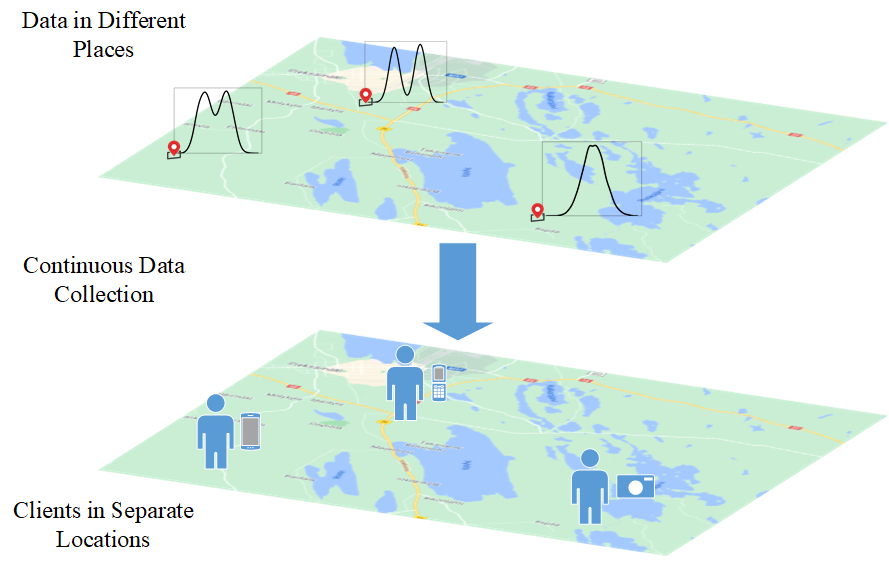
\includegraphics[height=6cm,width=8.6cm]{Fig1.png}
  \caption{The clients collect data from real world}
  \label{problem}
\end{figure}

Based on the aforementioned insights,  
we tackle the challenging real-scenarios-based federated
learning problem by selecting clients to participate in model
training through parameter prediction. We make several 
technical contributions:
% We propose a novel Federated framework estimation 
% based dynamic selection (FedDCS) whose central idea 
% is the parameter estimation based dynamic selection 
% mechanism. FedDCS allows the clients to join the 
% training freely, and we utilize the parameter estimation
% algorithm to dynamically select participants. Once the 
% client intends to join the FL, he needs
% to run the preset estimation algorithm and then send 
% the results (distribution parameters) to server, then
% the server will use the parameters to rebuild the 
% distribution model and compare it with the predetermined
% indicators to determine whether to accept or not.
% Moreover, since the act of collecting data is ongoing,
% we utilize Gaussian Mixture Model (GMM) to indicate
% the distribution of the local data each client holds.
% Note that the parameter estimation algorithm is only
% applicable for the condition that data follows GMM. 
% With the selection mechanism, FedDCS can screen out 
% clients which hold high quality data to participate 
% in the learning, and therefore acquire a better global model.
	
% We prove the convergence of estimation algorithm, 
% in limited rounds, this algorithm will converge 
% to a local maximum. Furthermore, we conduct 
% experiments to demonstrate the superior performance of FedDCS.
\begin{itemize}
    \item [1)]We propose a novel Federated Learning framework based on Dynamic 
    Client Selection method, namely FedDCS, whose central idea is
     the parameter estimation based dynamic selection mechanism.
      FedDCS allows the clients to join the training freely, 
      and we utilize the parameter estimation algorithm to select
       participants dynamically. To the best of our knowledge, this
        is the first work that combines parameters estimation and 
        dynamic selection mechanism to solve real-scene data-based Non-IID problem in FL. 
    \item [2)]We introduce Gaussian Mixture Model (GMM) to indicate 
    the distribution of real-world Non-IID data sets, and design an
     estimation algorithm to predict the parameters of GMM holds by clients.
      GMM can better clarify the continuously collected data. Moreover, 
      we introduce Intel SGX TEE to ensure data privacy and the authenticity of uploading data.
    \item [3)]We prove that the convergence of estimation algorithm,
    in limited rounds, this process will converge to a local maximum.
    \item [4)]We conduct extensive experiments on FedDCS: we test the convergence speed of the estimation algorithm and time loss of utilizing Intel SGX to execute estimation algorithm in different buffer sizes. The comparison experiment between FedAvg, FedSGD, and FedDCS demonstrates the superior performance of our framework.
\end{itemize}
The remainder of the paper is organized as follows. In Sec. 2, we review the related works. In Sec. 3, we introduce the preliminaries and definitions.
Modeling and the problem formulation will be introduced in Sec. 4.
We elaborate the FedDCS in Sec. 5. In Sec. 6, we conduct the convergence analysis of estimation algorithm. The simulations and evaluations are presented in Sec. 7. We make the conclusion in Sec. 8.
\section{Related Work}
Since FL is proposed in 2016 by google, centralized 
FL frameworks have been gradually improved. Federated 
learning framework FATE\cite{yang2019federated1} and TensorFlowFederated\cite{tensorflow2015-whitepaper} are the representatives. Leaf Project \cite{caldas2019leaf}
has provided multiple training environments which can simulate different
Non-IID and IID scenarios. According to the frameworks, a central server
is responsible for managing clients to accomplish machine learning tasks and coordinate the whole steps of 
algorithm. Each client keeps data in local storage
so that they can preserve the privacy. In centralized frameworks, all the selected nodes 
are supposed to send updates to central server, leading to communication 
congestion, and the limited bandwidth also slows the global model convergence.

To avoid the communication bottleneck, some researchers have proposed new 
frameworks. Pokhrel \textit{et al.}\cite{9079513} and Li \textit{et al.}\cite{li2020blockchain} have 
proposed a blockchain-based decentralized FL framework. Roy \textit{et al.}\cite{roy2019braintorrent}
proposed a peer-to-peer decentralized FL algorithm. 
Jeong \textit{et al.}\cite{jeong2018federated}, Itahara \textit{et al.}\cite{itahara2020distillation} and Li \textit{et al.}\cite{li2019fedmd} have
proposed knowledge distillation methods to minimize the 
communication overhead. In a decentralized FL framework, 
nodes are supposed to coordinate with each other to obtain the global model, 
and the model updates will be exchanged only between nodes. Without communicating 
with a server, clients can perform the whole process themselves. Although 
decentralized frameworks ease the communication pressure to a certain extent, 
privacy leakage, untrusted nodes and Non-IID data sets can drastically influence training performance.

Non-IID data has been a hot issue since FL was proposed. Non-IID data 
can significantly influence the training results\cite{yang2019federated2}, much work has been done.
FedProx\cite{li2020federated} works well on Non-IID, it dynamically adjusts the local 
training iterations of each round, aiming to reduce the communication pressure
and maximize the use of local computing resources. Zhao \textit{et al.}\cite{zhao2018federated} and Lu \textit{et al.}\cite{8843900} have proposed
 global sharing methods to provide a supplement 
for missing data, which aim to achieve faster convergence and higher global accuracy. 
Similarly, Federated Transfer Learning\cite{9076003} allows knowledge to be shared without compromising user privacy. 
Hsieh \textit{et al.}\cite{hsieh2020non} have presented 
SkewScout, which can control the communication frequency according to the data 
distribution offset. FedAMP\cite{huang2021personalized} is a framework 
that can satisfy individual model requirements. Differing from the conventional FL 
framework, FedAMP can customize self-adaptive modes, requiring clients to 
join in machine learning. SCAFFOLD\cite{karimireddy2020scaffold} is a 
new algorithm specialized for Non-IID data training, and it aims 
to improve training performance in client-shift circumstances.

Besides using share data set to fulfill the shifting clients, there are researches
focus on client selection. Nishio \textit{et al.}\cite{nishio2019client} focus on selecting 
clients with limited computational resources. Zhang \textit{et al.}\cite{zhang2021dynamic} propose a dynamic
fusion-based FL algorithm. Tuor \textit{et al.}\cite{tuor2020data} design a 
selection mechanism aiming to choose the relevant clients.

Unlike the existing work, our study explores selection mechanisms that do not require a local training model. Our method is particularly effective when it meets data sets collected from real scenarios, typically following Gaussian distribution. 
\section{Preliminaries and Definitions}
\subsection{Federated Learning Framework}
Centralized Federated Learning Frameworks have been proposed to achieve a satisfying situation by both user privacy security and machine learning efficiency. It consists of a server node and a series of clients. Federated Learning requires a central server to coordinate clients training a global model. In general, the server is responsible for dispensing the initial global model and aggerating updates from clients. While the server does not accumulate data from clients, the clients store data locally to preserve privacy. 

We denote machine learning model as $W$, to update $W$, clients perform SGD or other gradient descent algorithm, this process can be depicted by
\begin{align}
  W_{j}^{l+1} \gets W_{j}^{l} - \nabla F(W_{j},D_{j})
\end{align}
where $j$ represents client $j$, $e$ denotes the $e$-th iteration of local training and $F(W,D)$ means the SGD methods trains model with local data set $D$.

After each client finished local training, 
server executes global aggregation task. 
This process can be performed for serval epochs. Let $t$ denote global epochs, 
the fusion of global model can be calculated by
  \begin{align}
    W^{t+1} \gets \sum\limits_{j \in M} W^t_{j} 
  \end{align}
\subsection{Intel SGX Trusted Execution Environment}
Intel Software Guard Extensions\cite{costan2016intel} is a set of new instructions on recent model of intel CPUs,
which can confer reliable hardware-level security protection. Intel SGX can protect 
preselected codes and data fragments, developers can put data that need to be guarded into 
enclave. Enclave is a data storage zone that is isolated from software running outside of 
enclave. With the isolation protection, codes in enclave can keep confidentiality and 
integrity while the malicious software runs on the same system. Enclave memory is handled 
in plaintext only inside the CPU and is encrypted by the processor whenever it leaves so 
that even the OS can't access the data.

Intel SGX allows remote access to verify the software running in the enclave, and can 
communicate with it securely. And the software running in enclave can generate a report 
at times, which consists of supplementary data. The report is digitally signed with a hardware-level
 protected key. Remote computers have access to verify the report in order to prove 
that the measured software is running in Intel SGX enclave.

We assume the clients have access to Intel SGX Trusted Execution Environment, 
so that the preset programs can be executed in enclave without tampering.
Moreover, the central server can verify the 
reports generated by software remotely, and the clients can also keep data locally, 
which satisfies both sides.
\begin{figure}
    \centering
    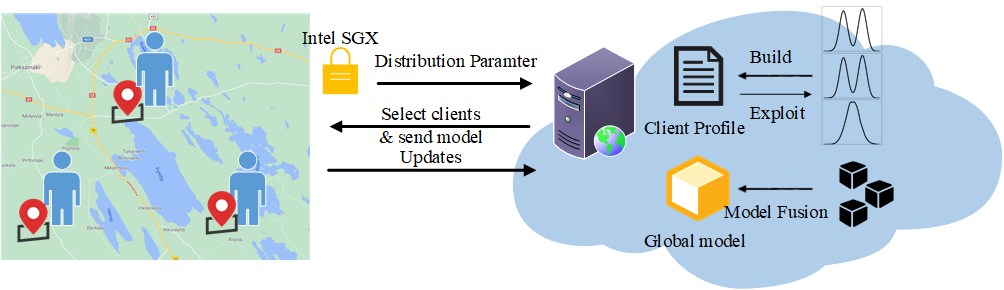
\includegraphics[height=2.5cm,width=8.7cm]{workflow.png}
    \caption{The workflow of FedDCS}
    \label{workflow}
\end{figure}
\subsection{Gaussian Mixture Model}
A mixture model is a probabilistic model for representing the presence of subpopulations 
in the overall population, it contains a series of complex data which belong to multiple 
regions with high probability mass. Data in mixture model are generated by randomly choosing
mixture components and sampling from the distribution which associated with this component.
Under this definition, we can do exact inference in the model.
Gaussian distribution is well known in statistics, it follows the probability function
  \begin{align}
    p(x|\theta) = \frac{1}{\sqrt{2\pi\sigma^{2}}}exp(-\frac{(x-u)^2}{2\sigma^2})
  \end{align}
where $x$ is univariate, and $u$ represents mean value or expectation of $x$, and $\sigma$ is standard 
deviation.
According to the previous definitions, we introduce Gaussian Mixture Model. Assuming a set of observation data 
$x_1,x_2,\dots,x_n$ which is sampled from $K$ single gauss models, and $\alpha_k$ is the
probability that observation data belongs to the $K$-th gauss model. $\phi (x|\theta_k)$ is the
probability of $K$-th gauss model. With parameters above, GMM follows probability density function:
  \begin{align}
    p(x|\theta) = \sum_{k=1}^{K}\alpha_k\phi(x|\theta_k)  
  \end{align}
for each single gauss model, $\theta$ represents the combination of parameters $u,\sigma$ and $\alpha$.


\section{modelling and  problem formulation}
Our objective is to achieve better performance on real-world-
based Non-identically distributed (Non-IID) data sets in 
FL and preserve client privacy in the same time.

Consider a real scenario where a series of clients
 $C = \left\{c_1,c_2,\dots, c_M \right\}$ are collecting data in different places
$P = \left\{P_1,P_2,\dots P_M \right\}$ and different time periods
$T = \left\{T_1,T_2,\dots T_K \right\}$. After the collection task is
finished, each client $c_j$ holds the data set $D_j$. We assume in
time period $T_k$ the subset of data set $D_j$ collected by client 
$c_j$ follows Gaussian distribution $p_k$, that is to say, each
data set $D_j$ is a combination of data from $T_1,T_2 \dots ,T_K$,
which follows $p_1,p_2, \dots, P_K$ respectively. Obviously, 
those data sets are Non-IID, in detailed depiction, they have a 
prior probability shifting problem \cite{kairouz2019advances}, which can result 
in sharply decrease of global model performance. Here we 
utilize GMM to describe the complex distribution, according 
to equation (4), the data set $D_j$ follows probability:
\begin{align}
  p(x|\theta) = \sum\limits_{k = 1}^{K} \alpha_k\cdot p_k
\end{align}
where $\alpha_k$ represents the ratio of $k$-th distribution to the total observed data $x$.

After finishing the data collecting, clients intend 
to join the collaborating machine learning task. As 
shown in figure 2, the server is supposed to take
over the entire process including selecting clients,
dispensing global models, and fuse global model. 
This procedure will iterate several times 
till the final convergence. Each client $c_j$ 
stores a data set $D_j$ locally and the server 
can't obtain any information about the collected data.
Under this circumstance, the server cannot screen out
the clients who hold the low-quality data sets, and thus 
the accuracy of global model drops drastically.

We dedicate efforts to improving the machine learning accuracy 
and archiving faster convergence under the above condition.


\section{FedDCS framework}
In this section, we propose a Federated Learning Framework FedDCS, which consists of Estimation Algorithm,
Intel SGX Trusted Execution Environment, Dynamic Selection Mechanism and Model Fusion Mechanism.

In order to obtain the data distribution of all clients which can enable the
server to evaluate the value of clients, FedDCS utilize Estimation algorithm 
to acquire the GMM parameters from the Intel SGX Enclave, which can preserve 
data privacy. Based on those augments, Dynamic Selection mechanism can screen
out the valuable data sets, which can facilitate the performance of machine
learning model. The details of above techniques will be elaborated in following sections. 
\begin{table}
\caption{Description of major notations}\label{tab2}
\begin{tabular}{c|m{6cm}}
\hline
Variable    & Description \\ \hline
$D,D_j$     & the data set, data set own by client $c_j$ \\ \hline
$C,c_j$     & the clients set, the $j$-th client. \\ \hline
$M,m$       &the number of total clients, number of selected clients \\ \hline
$n, N$      & the number of observation data samples, the number of total observation data \\ \hline
$k,K$       & the $k$-th Gaussian distribution, the number of all Gaussian distributions.  \\ \hline
$\alpha_k$ &the ratio of $k$-th distribution to total observed data.  \\ \hline
$\theta_k$ &the combination of parameters $u_k,\sigma_k , \alpha_k$.\\ \hline
$\phi (x|\theta)$ &the probability function of gauss model.\\ \hline
$x,x_i,X$ &the observation data samples,the $i$-th data sample of $x$, the observation data. \\ \hline
$Y$ &the hidden variable. \\ \hline
$Z$ &the complete data, which consists of $X$ and $Y$. \\ \hline
$Q(\theta)$ &the estimation-step function of estimation algorithm.\\ \hline
$L(\theta|x)$ &the likelihood function of GMM. \\ \hline
$t$ &the $t$-th round of global epoch. \\ \hline
$l$ &the $l$-th iteration of local training \\ \hline
$W,W_j$ &the machine learning model, the machine learning model own by client $c_j$ \\ \hline
$\delta, \delta_s$  &the difference between current model and standard model, the threshold of $\delta$. \\ \hline
$p,p_k$   & the probability function, the probability function of $k$-th component in mixture model. \\ \hline
\end{tabular}
%\vspace{-0.1in}
\end{table}
\subsection{Estimation Algorithm}
GMM is a generation model, it assumes that data are generated from multiple
Gaussian distributions. In this paper we offer each distribution a weight 
$\alpha_k$, and when data generate, GMM randomly select a distribution according
to the $\alpha_k$, then, GMM creates data copies which follow chosen distributions. 

According to the previous definition, server can't acquire the GMM parameters 
directly, therefore, we utilize the estimation algorithm to predict those arguments.
 To achieve the prediction task, we have to seek the solution for equation (5).
We firstly introduce likelihood function, assuming we have samples $X = \left\{x_1,x_2,\dots, x_n \right\}$ from
the same distribution and they are 
independent identically distributed, following probability $p$. 
So we get joint probability density function
$L(\theta|x) = p(x|\theta) = \prod_{i = 1}^{n} p(x_i|\theta)$
which is regarded as the likelihood function of $\theta$.

Since the value of function $L$ can change with $\theta$, we utilize
Maximum Likelihood Estimation $\theta^* = argmax  L(\theta|X)$ to figure out the optimal value
of $\theta$ to maximize function $L$.
To make the equation computable, we change it to 
   $ \ln (L(\theta|x)) = \sum_{i = 1}^{n} \ln p(x_i|\theta)$
and to seek the max value of $L$, we take the derivative of log-likelihood function
   $ \frac{\partial}{\partial \theta} \ln L(\theta \mid X)=0$.

According to the previous equations, the log likelihood function of GMM can be written as:
  \begin{align}
    \ln (L(\theta|X)) = \ln \prod_{i=1}^{N}p(x_i|\theta) = \sum_{i=1}^{N}\ln[\sum_{k=1}^{K}\alpha_k p_k(x_i|\theta_k)] 
  \end{align}

Obviously, it's quite hard seeking the max value by directly
deriving the log likelihood function, but if we know which 
distribution the observed data $x_i$ stems from, the equation (6) 
can be solved. We introduce a hidden variable $Y = y_1,y_2,\dots ,y_N$,
and $y_i \in 1,2,\dots ,K$, where $y_i = k$ 
indicates thta the sample $x_i$ originates from distribution $k$. 
$\ln(L)$ can be written as
  \begin{align}
    \ln (L(\theta|x,y)) = \ln \prod_{i = 1}^{N} p(x_i,y_i|\theta) = \sum_{i=1}^{N} \ln(\alpha_{y_i} p_{y_i}(x_i|\theta_{y_i}))
  \end{align}

We denote $Z = (X,Y)$ to represent the complete data, $X$ is the observation data and $Y$
is the hidden variable. $p = (y|x,\theta)$ is the density of hidden
variable given the observed data $X$. 
  \begin{align}
    p(y|x,\theta) = \frac{p(z|\theta)}{p(x|\theta)} = \frac{p(x,y|\theta)}{p(x|\theta)}
  \end{align}

  We use iterative method to find the max value of $L(\theta|X)$ and denote $\theta^e$ as $e$-th
round iteration optimal parameter of function as $L(\theta|X)$.
We define $Q(\theta|\theta^e)$ as the expectation of loglikelihood 
function under the condition of observation data $X = x_1,x_2,\dots , x_n$ as follows
  \begin{align}
    Q(\theta|\theta^{(e)}) &= E[\log L(\theta|Z)|x,\theta^{(e)}] \notag  \\
& = \int [\log p(z|\theta)]p(y|x,\theta^{(e)} \,dy 
  \end{align}

While the observation data $X$ 
is given, we are going to solve the equation about $Y$. We 
seek the condition expectations on $Y$ and obtain an equation
 only related to $\theta$. 
  
The estimation algorithm begins with $\theta^{(0)}$, and executes
 the iterations of Estimation step and Maximization step.
  estimation step aims to calculate the conditional expectation of 
$Q(\theta|\theta^{(e)})$ and Maximization step aims to maximum $Q(\theta|\theta^{(e)})$.
Assume we have gotten $\theta^{(e-1)}$ in $e-1$-th iteration,
 in GMM we get
 \begin{align}
  \theta^{(e-1)} = (\alpha_1^{(e-1)},\dots , \alpha_K^{(e-1)},\theta_1^{(e-1)},\dots,\theta_K^{(e-1)}) \notag
 \end{align}

  According to equation (9), the estimation step is:
\begin{align}
& Q(\theta|\theta^{(e-1)}) = E[\ln (L(\theta|X,Y))] \notag  \\
& =\sum\nolimits_{y} \ln (L(\theta|X,y)) p(y|X,\theta^{(e-1)}) \notag  \\
& =\sum \nolimits_{y} \sum\nolimits_{i=1}^{N} \ln (\alpha_{y_i} p_{y_i},(x_i|\theta_{y_i})) p(y|x_i,\theta^{(e-1)})
\end{align}

Since we already know that $ p(y_i = k|x_i,\theta^{(e-1)})$ represent the 
probability of sample $x_i$ originating 
from $k$-th distribution, the equation (10) can be written as:
% \sum_{k=1}^{K} \sum_{i=1}^{N} \ln (\alpha_k p_k (x_i|\theta_k)) p(k|x_i,\theta^{e-1}) \notag  \\ 
\begin{align}
  &Q(\theta|\theta^{(e-1)}) = \sum_{k=1}^{K} \sum_{i=1}^{N} \ln (\alpha_k p_k (x_i|\theta_k)) p(k|x_i,\theta^{e-1}) \notag  \\ 
  &=\sum_{k=1}^{K} \sum_{i=1}^{N} \ln (\alpha_k) p(k|x_i,\theta^{(e-1)}) \notag  \\
  & +\sum_{k=1}^{K} \sum_{i=1}^{N} \ln (p_k(x_i|\theta_k)) p(k|x_i,\theta^{(e-1)}) 
\end{align}
Based on Bayes Theorem, $p(k|x_i,\theta^{(e-1)}) $ can be written as 
\begin{align} 
p(k|x_i,\theta^{(e-1)}) 
% = \frac{p(k,x_i|\theta_{k}^{e-1})}{\sum_{k^{'}=1}^{K} p(k^{'},x_i|\theta_{k^{'}}^{(e-1)})} 
= \frac{p_k(x_i|\theta_{k}^{e-1})}{\sum_{k^{'}=1}^{K} p_{k}^{'}(x_i|\theta_{k^{'}}^{(e-1)})}
\end{align}
and $p(k,x_i|\theta_{k}^{(e-1)})$ can be calculated by equation (8).

Maximization step utilizes derivation to seek the optimum parameters, 
\begin{small}
\begin{align}
  &\frac{\partial Q\left(\theta \mid \theta^{(e-1)}\right)}{\partial \mu_{k}}
    =\frac{\partial}{\partial \mu_{k}}\left[\sum_{i=1}^{N} \ln \left(p_{k}\left(x_{i} \mid \theta_{k}\right)\right) p\left(k \mid x_{i}, \theta^{(e-1)}\right)\right] \notag \\
    &=\frac{\partial}{\partial \mu_{k}}\left[\sum_{i=1}^{N}\left(\ln \left(\frac{1}{\sqrt{2 \pi \sigma_{k}^{2}}}\right)-\frac{\left(x_{i}-\mu_{k}\right)^{2}}{2 \sigma_{k}^{2}}\right) p\left(k \mid x_{i}, \theta^{(e-1)}\right)\right] \notag \\
    &=\sum_{i=1}^{N}\left[\frac{1}{\sigma_{k}^{2}}\left(x_{i}-\mu_{k}\right) p\left(k \mid x_{i}, \theta^{(e-1)}\right)\right] \notag \\
    &=\frac{1}{\sigma_{k}^{2}} \sum_{i=1}^{N}\left(x_{i} p\left(k \mid x_{i}, \theta^{(e-1)}\right)\right)-\frac{\mu_{k}}{\sigma_{k}^{2}} \sum_{i=1}^{N} p\left(k \mid x_{i}, \theta^{(e-1)}\right) =0 
\end{align}
\end{small}
from equation (13), we get $u_k$, and similar, we derive $Q(\theta|\theta^{e-1})$ with respect to $\sigma_k^{2}$. 
We get $u_k$ and $\sigma_k^{2}$ as follows
\begin{align}
  &\mu_{k}=\frac{\sum_{i=1}^{N}\left(x_{i} p\left(k \mid x_{i}, \theta^{(e-1)}\right)\right)}{\sum_{i=1}^{N}\left(p\left(k \mid x_{i}, \theta^{(e-1)}\right)\right)}\\
  &\sigma_{k}^{2}=\frac{\sum_{i=1}^{N}\left(\left(x_{i}-\mu_{k}\right)^{2} p\left(k \mid x_{i}, \theta^{(e-1)}\right)\right)}{\sum_{i=1}^{N}\left(p\left(k \mid x_{i}, \theta^{(e-1)}\right)\right)}
\end{align}

Note that $\alpha_k$ can't be calculated by using derivation directly, we introduce Lagrange multiplier $\sum_{k=1}^{K} \alpha_k -1$,
and we get equation as follows
\begin{small}
\begin{align}
  \begin{aligned}
    & \frac{\partial}{\partial \alpha_{k}}\left[Q\left(\theta \mid \theta^{(e-1)}\right)+\lambda\left(\sum_{k=1}^{K} \alpha_{k}-1\right)\right]  \\
    =& \frac{\partial}{\partial \alpha_{k}}\left[\sum_{k=1}^{K} \sum_{i=1}^{N} \ln \left(\alpha_{k}\right) p\left(k \mid x_{i}, \theta^{(e-1)}\right)+\lambda\left(\sum_{k=1}^{K} \alpha_{k}-1\right)\right]   \\
    =& \frac{1}{\alpha_{k}} \sum_{i=1}^{N} p\left(k \mid x_{i}, \theta^{(e-1)}\right)+\lambda=0
  \end{aligned}
\end{align}
\end{small}
finally we get:
\begin{align}
  \alpha_{k}=\frac{\sum_{i=1}^{N}\left(p\left(k \mid x_{i}, \theta^{(e-1)}\right)\right)}{N}
\end{align}
\subsection{Dynamic Selection Mechanism}
We obtain parameters from estimation algorithm in previous section,
with those parameters, a dynamic selection mechanism will be designed. 

Firstly, we take effort dedicated to fitting parameters $u, \sigma$ and $\alpha$
to a more general one $\delta $, and a preset value $\delta_s$, since $u$ and $\sigma $
stems from GMM, this mechanism will rebuild a GMM on the basis of 
those data, and calculate a difference of current distribution and 
standard distribution. In detailed depiction, this mechanism will compute
 the difference of the occurring frequency between label $i$ and standard ones.

Argument $\delta_s$ set a threshold for selecting clients, \textit{i}.\textit{e}.,
we only choose nodes whose $\delta < \delta_s$, and selected clients will join the training,
then perform FedAvg and gather all local models to get a global model. The clients can 
execute the estimation algorithm once they have finished collection tasks, 
and the server can centralized processes the received parameters.  
The argument $\delta_s$ can be changed in a predetermined range so that the server can set 
the severity if the selected requirements. The Algorithm 1 gives an explicit description of the workflow.

As server can't acquire samples from the nodes, 
the rebuilding of GMM depends entirely on the parameters
calculated in previous section. We set random number $n<N$ as
the sample space, where $N$ represents the total data size,
and $n$ must be greater than 500, or the rebuilt model would be quite different from the original one. 
\begin{algorithm}[t]
  \caption{Dynamic Selection Mechanism}
  \SetAlgoLined
  \KwIn{$M$ clients, each hold a set of private data. One Server}
  \KwOut{$m$ selected clients}
  % \KwData{}
  % \KwResult{}
  % Initialization\;
  \KwData{inital model $W_g$ and preset threshold $\delta_s$}

  \For {client $c_j$ in $M$ Clients}{
    run estimation algorithm in SGX Enclave;

    upload parameter $\theta_j$ to Server;

    wait for response;
  }
  \While{server get each $\theta_j$}{
    rebuild GMM $G$ with $\theta_j$;

    calculate $\delta_j$ from $G_j$ ($G_j \to \delta_j$);

    \eIf{$\delta_j < \delta_s$}{
      send initial model $M_g$ to client $j$; 
    }{
      send rejection message to client $j$;
    }
  }
  \label{selection}
\end{algorithm}
\subsection{Model Fusion}
In each epoch, the server node aggerates information and performs selection mechanism, then, 
those nodes will execute local training and run FedAvg algorithm to gather models and
 fuse into a global one. We make a detailed description of this process in Algorithm 2.

 \begin{algorithm}[t]
  \caption{Model Fusion}
  \SetAlgoLined
  \KwIn{$M$ clients, each hold a set of private data $D_j$. One Server hold a global model.}
  \KwOut{a trained global model $W_g$}
  Initialization;
  
  From Algorithm 1, get selected clients $C_m$;
  
  Server send initial model $W_g$ to $C_m$;

  \For{each round $t = 1,2,\dots $}{
    \For{each client $c_j \in C_m$}{
      $W^{k+1}_{j} \gets W_j^k - \nabla F(W,D_j)$
    }
    $W_g^t = \sum_{j = 1}^{m} \frac{1}{m} W_j $ 
  }
    \label{FedAvg}
\end{algorithm}

Note that in order to match the dynamic selection mechanism, once the client is chosen, 
the central server will not stop the current machine learning task, but send the last updates
to the selected clients in the next epoch. Moreover, the Server only dispense initial parameters to the selected node,
And also, only the selected nodes execute training works and upload models, which 
saves the bandwidth, increases spectrum efficiency and decreases communication pressure. 
In addition, the selection mechanism doesn't require any local computation so that the 
unselected nodes can save computing resources. 

\section{convergence analysis of estimation algorithm}
In this section, we analyze the convergence of estimation algorithm.
\begin{theorem}
Suppose that $P = \left\{p_1,p_2,\dots ,p_n\right\}$ 
and $Q = \left\{q_1,q_2,\dots ,q_n\right\}$ are two probability distributions.
The following inequality holds:
\begin{align}
    -\sum_{i=1}^{n}p_i \log p_i \le -\sum_{i=1}^{n}p_i \log q_i
\end{align}
the inequality changes to equality under the condition that if and only if  $p_i = q_i$
\end{theorem}
\begin{proof}
    \begin{align}
    &0 \ge \sum_{i=1}^{n}p_i \log q_i - \sum_{i=1}^{n}p_i \log p_i \notag \\
    &= \sum_{i=1}^{n} p_i \log (q_i/p+i)
    \end{align}
    according to $\ln (x) \le x-1$, the equal sign holds if and only if $x = 1$ , 
    the equation changes to:
    \begin{align}
    &\sum_{i=1}^{n} p_i \log (q_i/p+i) \ge \sum_{i=1}^{n} p_i \log (q_i/p_i-1) \notag \\
    &= \sum_{i=1}^{n} (q_i-p_i) = \sum_{i=1}^{n} q_i - \sum_{i=1}^{n} p_i = 0 \Longleftrightarrow q_i = p_i
    \end{align}
    \end{proof}
\begin{theorem}
$f(x), g(x)$ is the given probability distribution that has the same support.
\begin{align}
    H(f \mid g)=\int \log \left(\frac{g(x)}{f(x)}\right) g(x) d x \notag
\end{align}
and we get:
\begin{align}
    H(f|g) \le 0, "=" \Longleftrightarrow f(x) = g(x) \notag
\end{align}
\end{theorem}
\begin{proof}
\begin{align}
    &H(f|g) = \int \log (\frac{g(x)}{f(x)}) g(x) \,dx \notag \\
    & \ge \int (\frac{f(x)}{f(x)}-1)g(x) \,dx   \notag \\
    & = -\int f(x) \,dx + \int g(x) \,dx = 0
\end{align}
\end{proof} 
\begin{theorem}
Assume we get the estimated parameters $\left\{\theta^{e} \right\}$, 
and each maximization step increases the value of loglikelihood function $L(\theta|x)$
\begin{align}
    \log (p(x|\theta^{(e+1)})) \ge \log(p(x|\theta^{(e)}))
\end{align}
\end{theorem}

\begin{proof}
According to equation (8) and equation (9), we get:
    \begin{align}
    \log (p(z|\theta)) + c &= \log (p(x|\theta)) + \log(p(y|x,\theta)) + c \notag \\
    Q(\theta|\theta^{(e)}) &= \int_{Y} \left[\log(p(z|\theta))\right]p(y|x,\theta^{(e)}) d y \notag
    \end{align}

so we can get the following equations:
\begin{small}
    \begin{align} 
   & Q(\theta|\theta_{e})\! =  \! \int_{Y}\left(\log(p(x|\theta^{(e)}))\!+\!\log(p(y|x,\theta))\right) 
    \log(p(y|x,\theta^{(e)})) d y \notag\\
   & =\log(p(x|\theta^{(e)}))+\int\left[\log(p(y|x,\theta))\right] \log(p(y|x,\theta^{(e)}))d y \notag \\
   & \log(p(x|\theta^{(e+1)})) - \log(p(x|\theta^{(e)})) = Q(\theta|\theta^{(e+1)})-Q(\theta|\theta^{(e)}) \notag \\
   &  + \int \log \left(\frac{\log(p(y|x,\theta^{(e)}))}{\log(p(y|x,\theta^{(e+1)}))}\right) \log(p(y|x,\theta^{(e)})) d y 
    \end{align}
\end{small}
according to equation (22) and (23), we know that $\Delta Q(\theta^{(e+1)}|\theta^{(e)},X) \ge 0$. 
On the basis of Theorem2, we get :
    \begin{align}
    \int \log \left(\frac{\log(p(y|x,\theta^{(e)}))}{\log(p(y|x,\theta^{(e+1)}))}\right) \log(p(y|x,\theta^{(e)})) d y \ge 0 \notag \\
    \end{align}
\end{proof}

From Theorem3 we know the EM algorithm will finally converges 
to a global or local maximum, the parameter sequence 
$\Theta = \left\{\theta^{(1)},\theta^{(2)},\dots, \theta^{(e)}\right\}$ 
will eventually converges to the maximum likelihood estimation.
\section{Performance Evaluation}
In this section, we evaluate the performance of FedDCS and 
compare it with the popular Federated Learning algorithm, FedAvg and FedSGD. 
To make our experiment more comprehensive, we utilize two kind of CNN networks 
and three kinds of data sets to test the performance of FL framework.
\subsection{Environment Setting}
\subsubsection{Data Setting}
\begin{table}
    \caption{Time Loss of SGX in Different Buffer Size}
    \begin{tabular}{|c|c|c|l|}
    \hline
    \textbf{Buffer Size}           & \textbf{20kb}        & \textbf{10mb}        & \multicolumn{1}{c|}{\textbf{20mb}}       \\ \hline
    \textbf{CPU Cycles (StartUp)}  & $1.43 \times 10^{3}$ & $1.7 \times 10^{8}$  & \multicolumn{1}{c|}{$6.9 \times 10^{8}$} \\ \hline
    \textbf{CPU Cycles (ShutDown)} & $3 \times 10^{2}$    & $1.5 \times 10^{7}$  & \multicolumn{1}{c|}{$2.1 \times 10^{7}$} \\ \hline
    \textbf{Buffer Size}           & \textbf{40mb}        & \textbf{160mb}       &                                          \\ \hline
    \textbf{CPU Cycles (StartUp)}  & $1.3 \times 10^{9}$  & $5.25 \times 10^{9}$ &                                          \\ \hline
    \textbf{CPU Cycles (ShutDown)} & $4.13\times 10^{7}$  & $1.4 \times 10^{8}$  &                                          \\ \hline
    \end{tabular}
    \end{table}
    
We utilize CIFAR-10 and MNIST data sets to 
verify the performance of FedDCS. CIFAR-10 data set is a collection of
 images that are commonly used to train machine learning algorithm, 
 which contains 60,000 32*32 images in 10 different classes, 
 and the images are 3-channel RGB color ones. Similarly, 
 MNIST is a large database of handwritten digits $0$ to $9$ 
 and it contains 60,000 training images and 10,000 testing images.
Those images are 28*28 one channel (black and white). 
To simulate the real scene, we 
create 10 clients in this experiment, each holds a set of images. 
While those data are Non-IID, they follow GMM. For each kind of data set,
we randomly choose a series of normal distribution parameters and assign 
them to clients. We assume each client owns a GMM data set which 
consists of three Gaussian distributions. 
The unstableness catastrophically destroys the performance of FedAvg 
and also significantly influences local model training.

    Let us take CIFAR-10 for example to introduce how we apply the Non-IID data setting.
We firstly random generate a series of normal distribution parameters
$\theta_i = \left\{ u,\sigma ,\alpha \right\}$ and sample from CIFAR-10 with $\theta$. 
The sample categories are serialized as the one-hot form, 
number 0-9 corresponds to the category of CIFAR-10. 
Then we construct a GMM based on the three selected Gaussian distributions.
For convenience of computation, each distribution holds the same size of image sets, 
in different data sets, the set size can vary from 600 to 6000.
\begin{figure}
    \centering
    \includegraphics[height=6.67cm,width=8cm]{EM_PNG.png}
    \caption{Estimation Algorithm Loss}
    \label{em}
\end{figure}

\begin{figure*}[!t]
  %\subfigure[pic1.]{
  % \begin{minipage}[t]{0.25\linewidth}
  % \centering
  % %\subfigure[\label{revenue-regret-KN}Revenue and regret]{\includegraphics[width=0.99\textwidth]{reven_regret_kn.eps}}%\hspace{0.01in}
  % \includegraphics[width=0.99\textwidth]{EM_PNG.png}
  % \vspace{-0.2in}
  % \caption{}}\label{fig:revenue-regret-CMAB-KN-2}\vspace{-0.15in}
  % \end{minipage}%
  % %}%
  \begin{minipage}[t]{0.75\linewidth}
  \centering
  \subfigure[\label{fig:profit_c_kn-2}MNINST with AlexNet]{\includegraphics[width=0.33\textwidth]{MNIST_AlexNet_PNG.png}}%\hspace{0.01in}
  \subfigure[\label{fig:profit_p_kn-2}MNINST with LeNet-5]{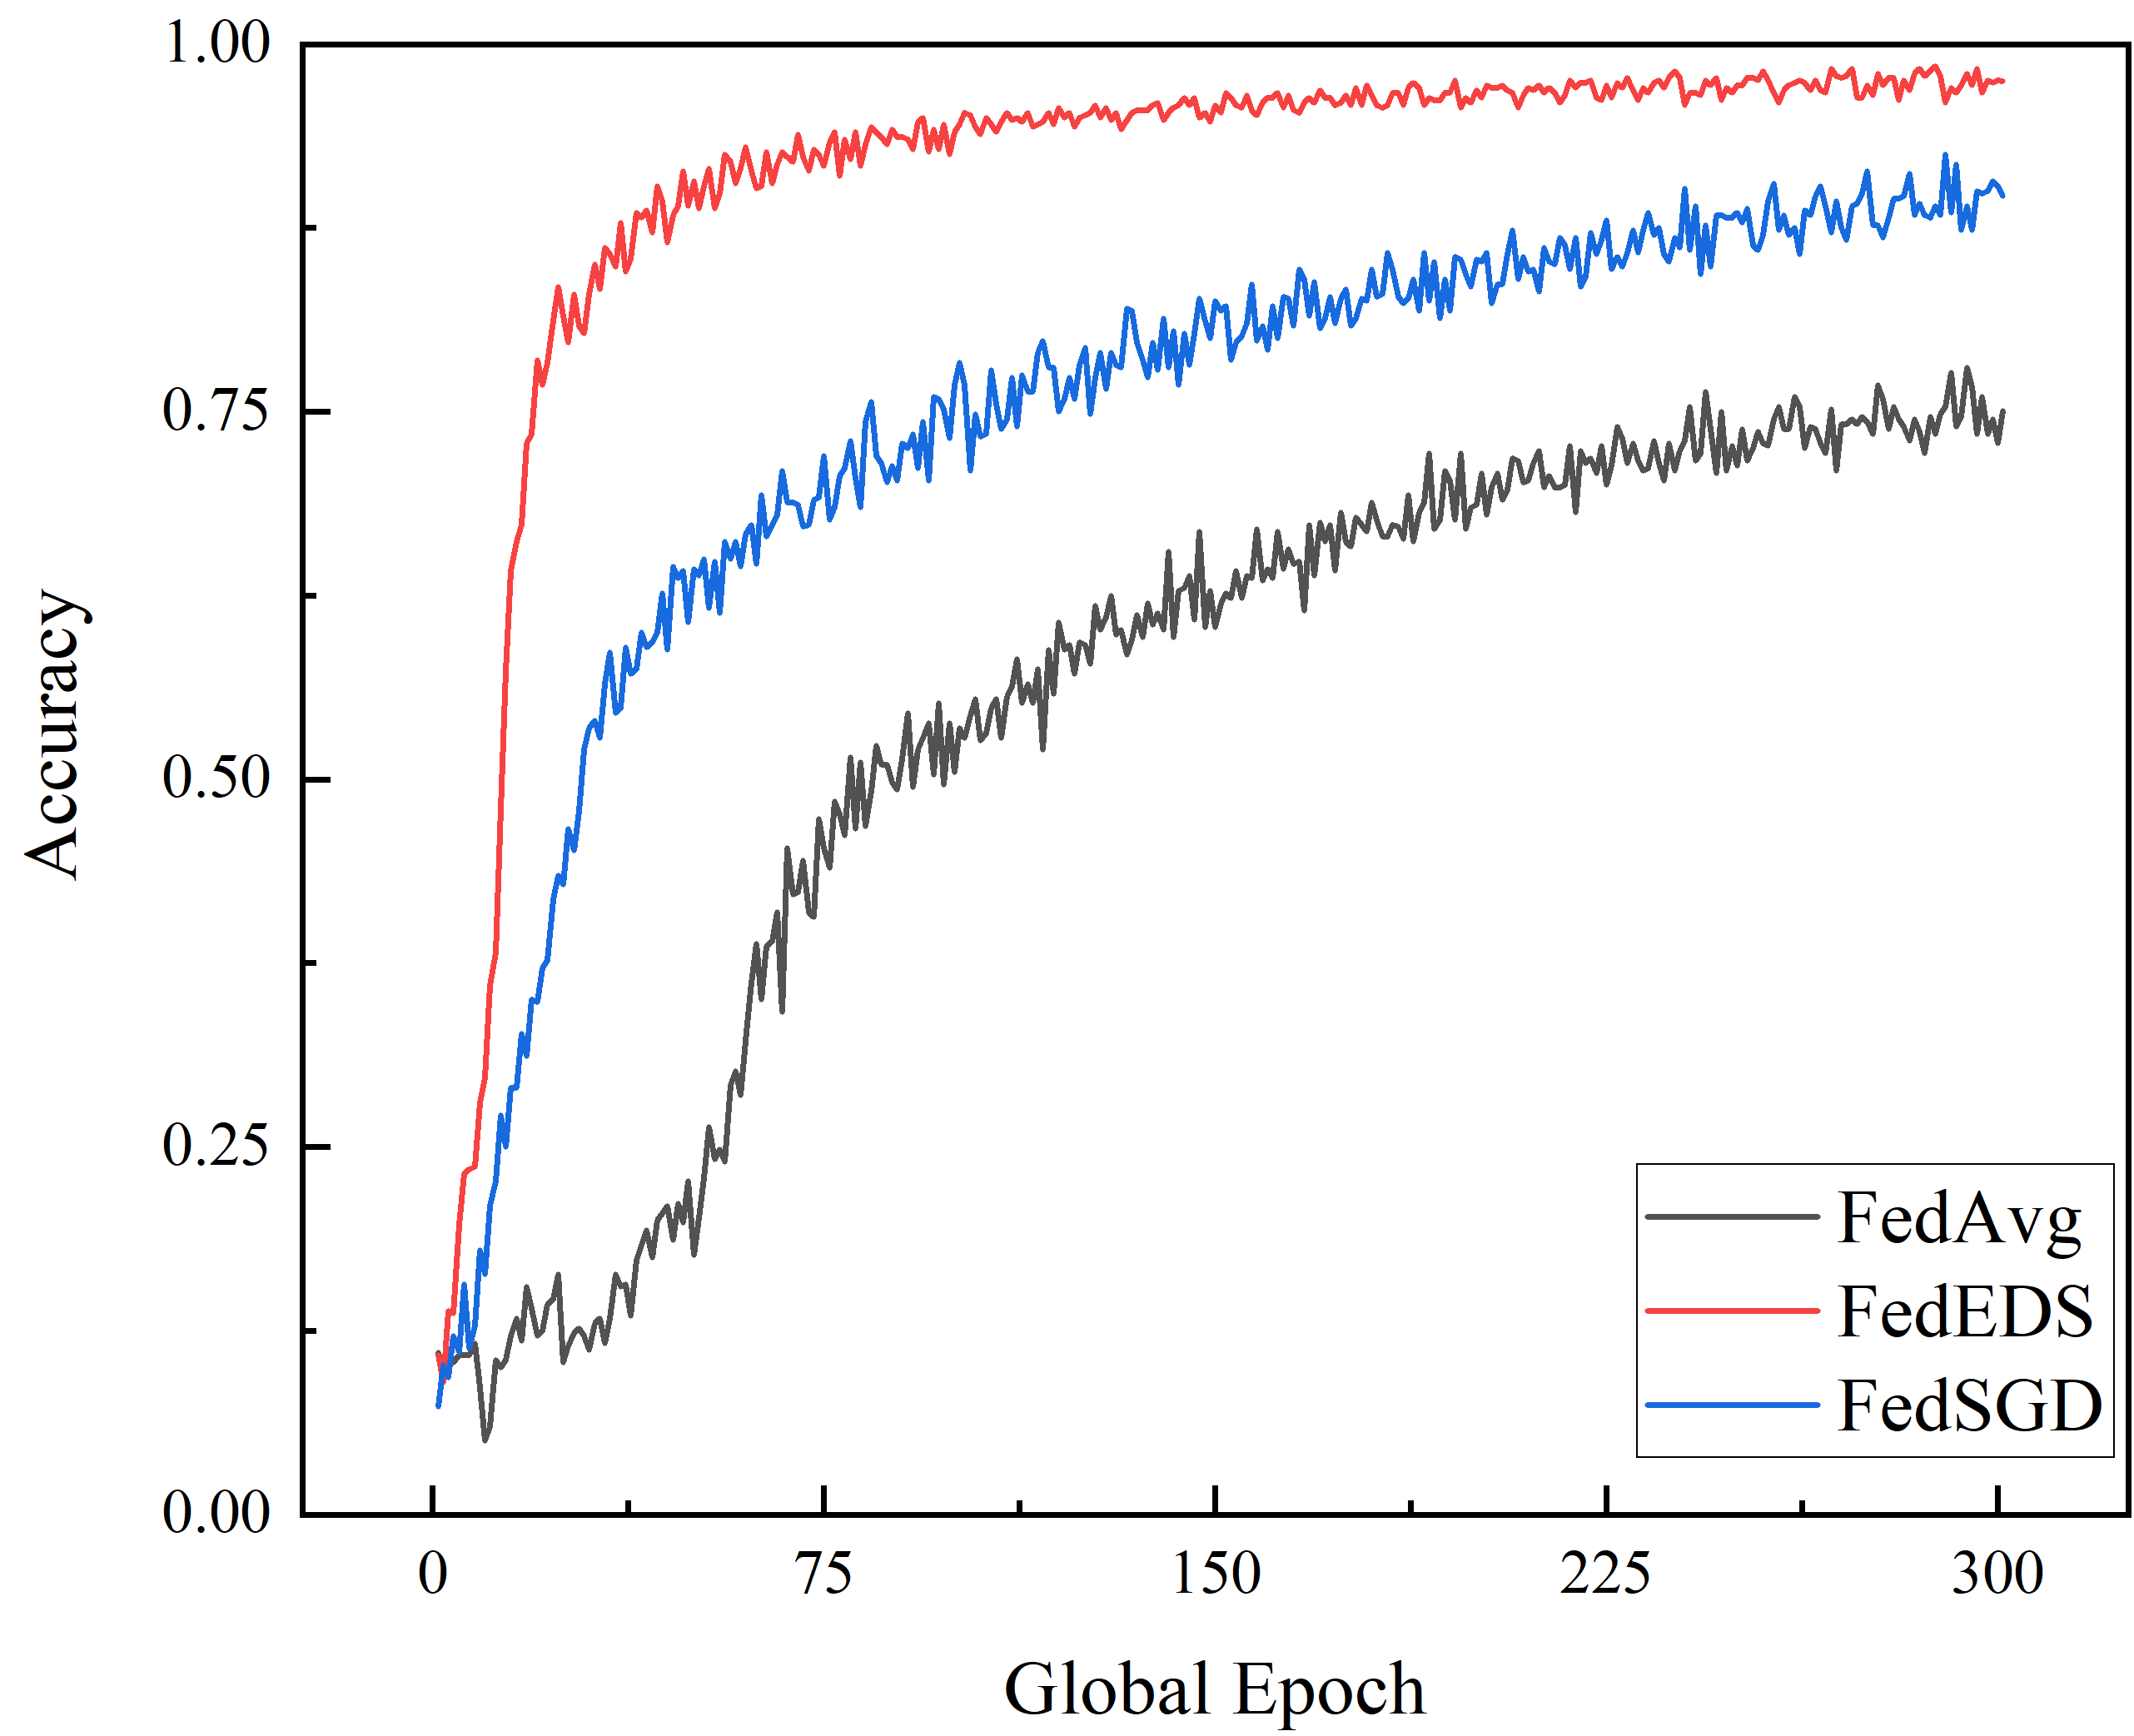
\includegraphics[width=0.33\textwidth]{MNIST_LeNet_PNG.png}}%\vspace{-0.01in}
  \subfigure[\label{fig:profit_s_kn-2}CIFAR-10 with AlexNet]{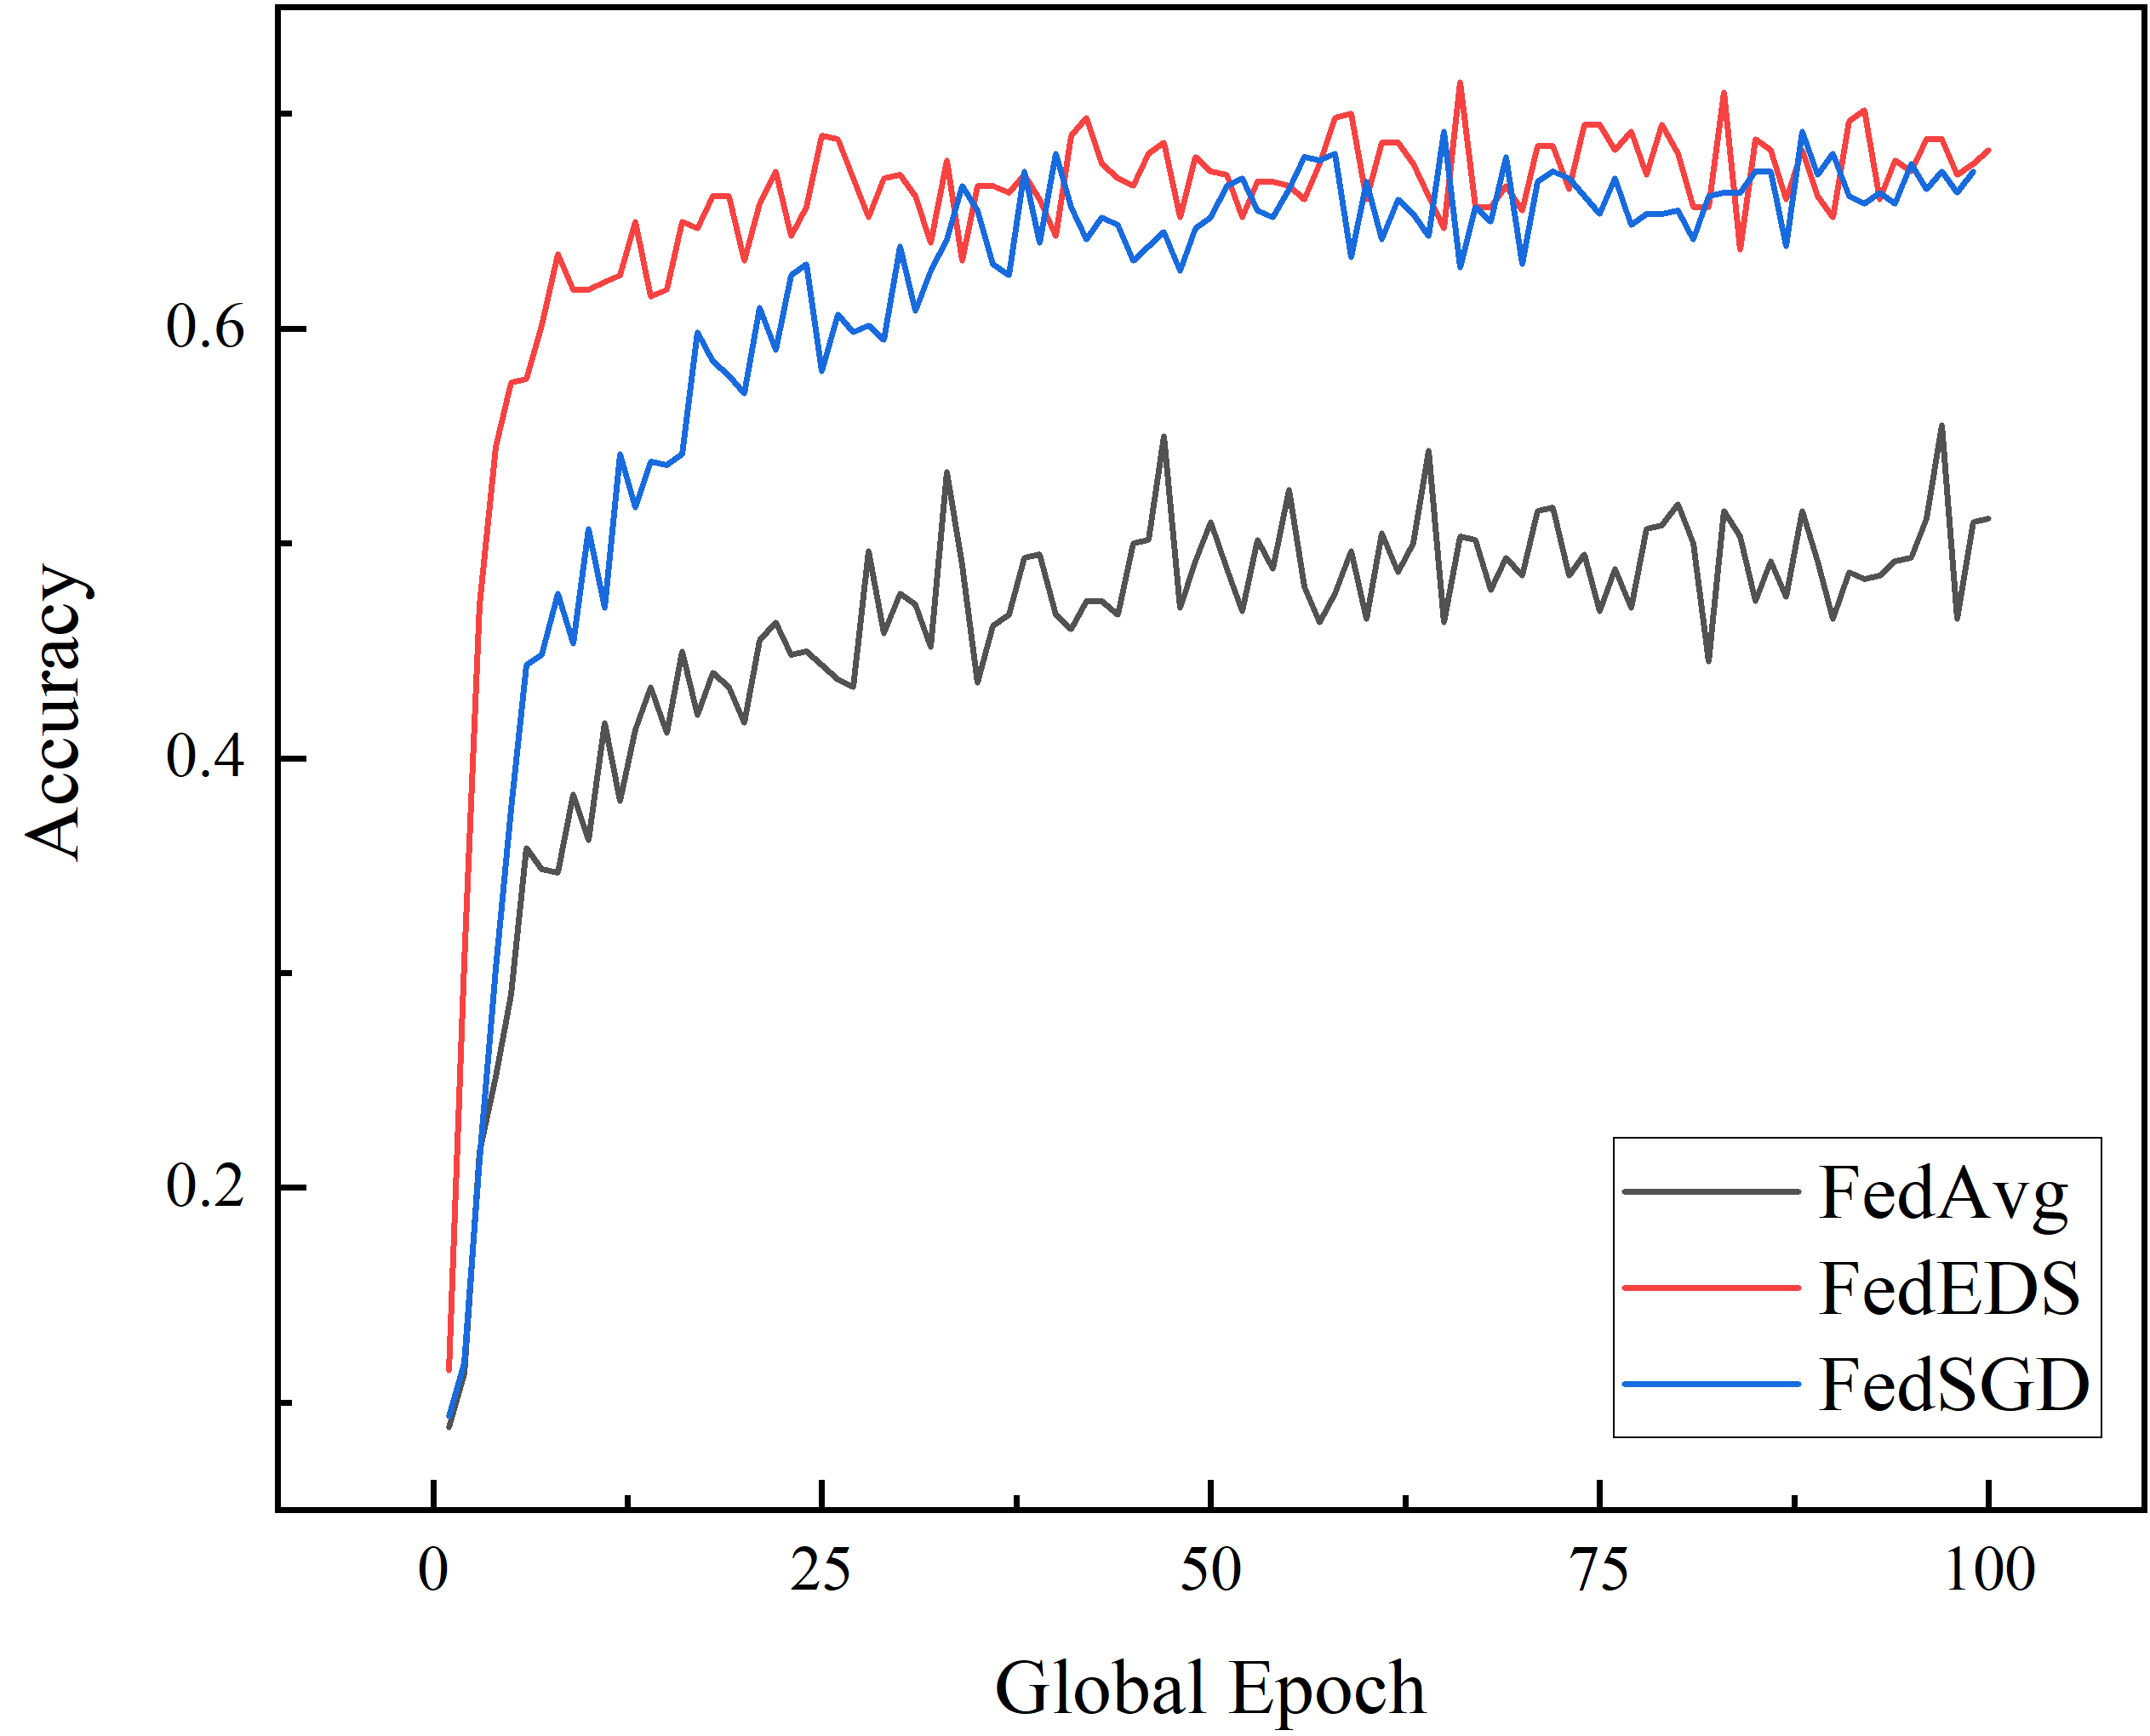
\includegraphics[width=0.33\textwidth]{CIFAR10_AlexNet_PNG.png}}%\vspace{-0.01in}
  \subfigure[\label{fig:profit_c_kn-3}CIFAR-10 with LeNet-5]{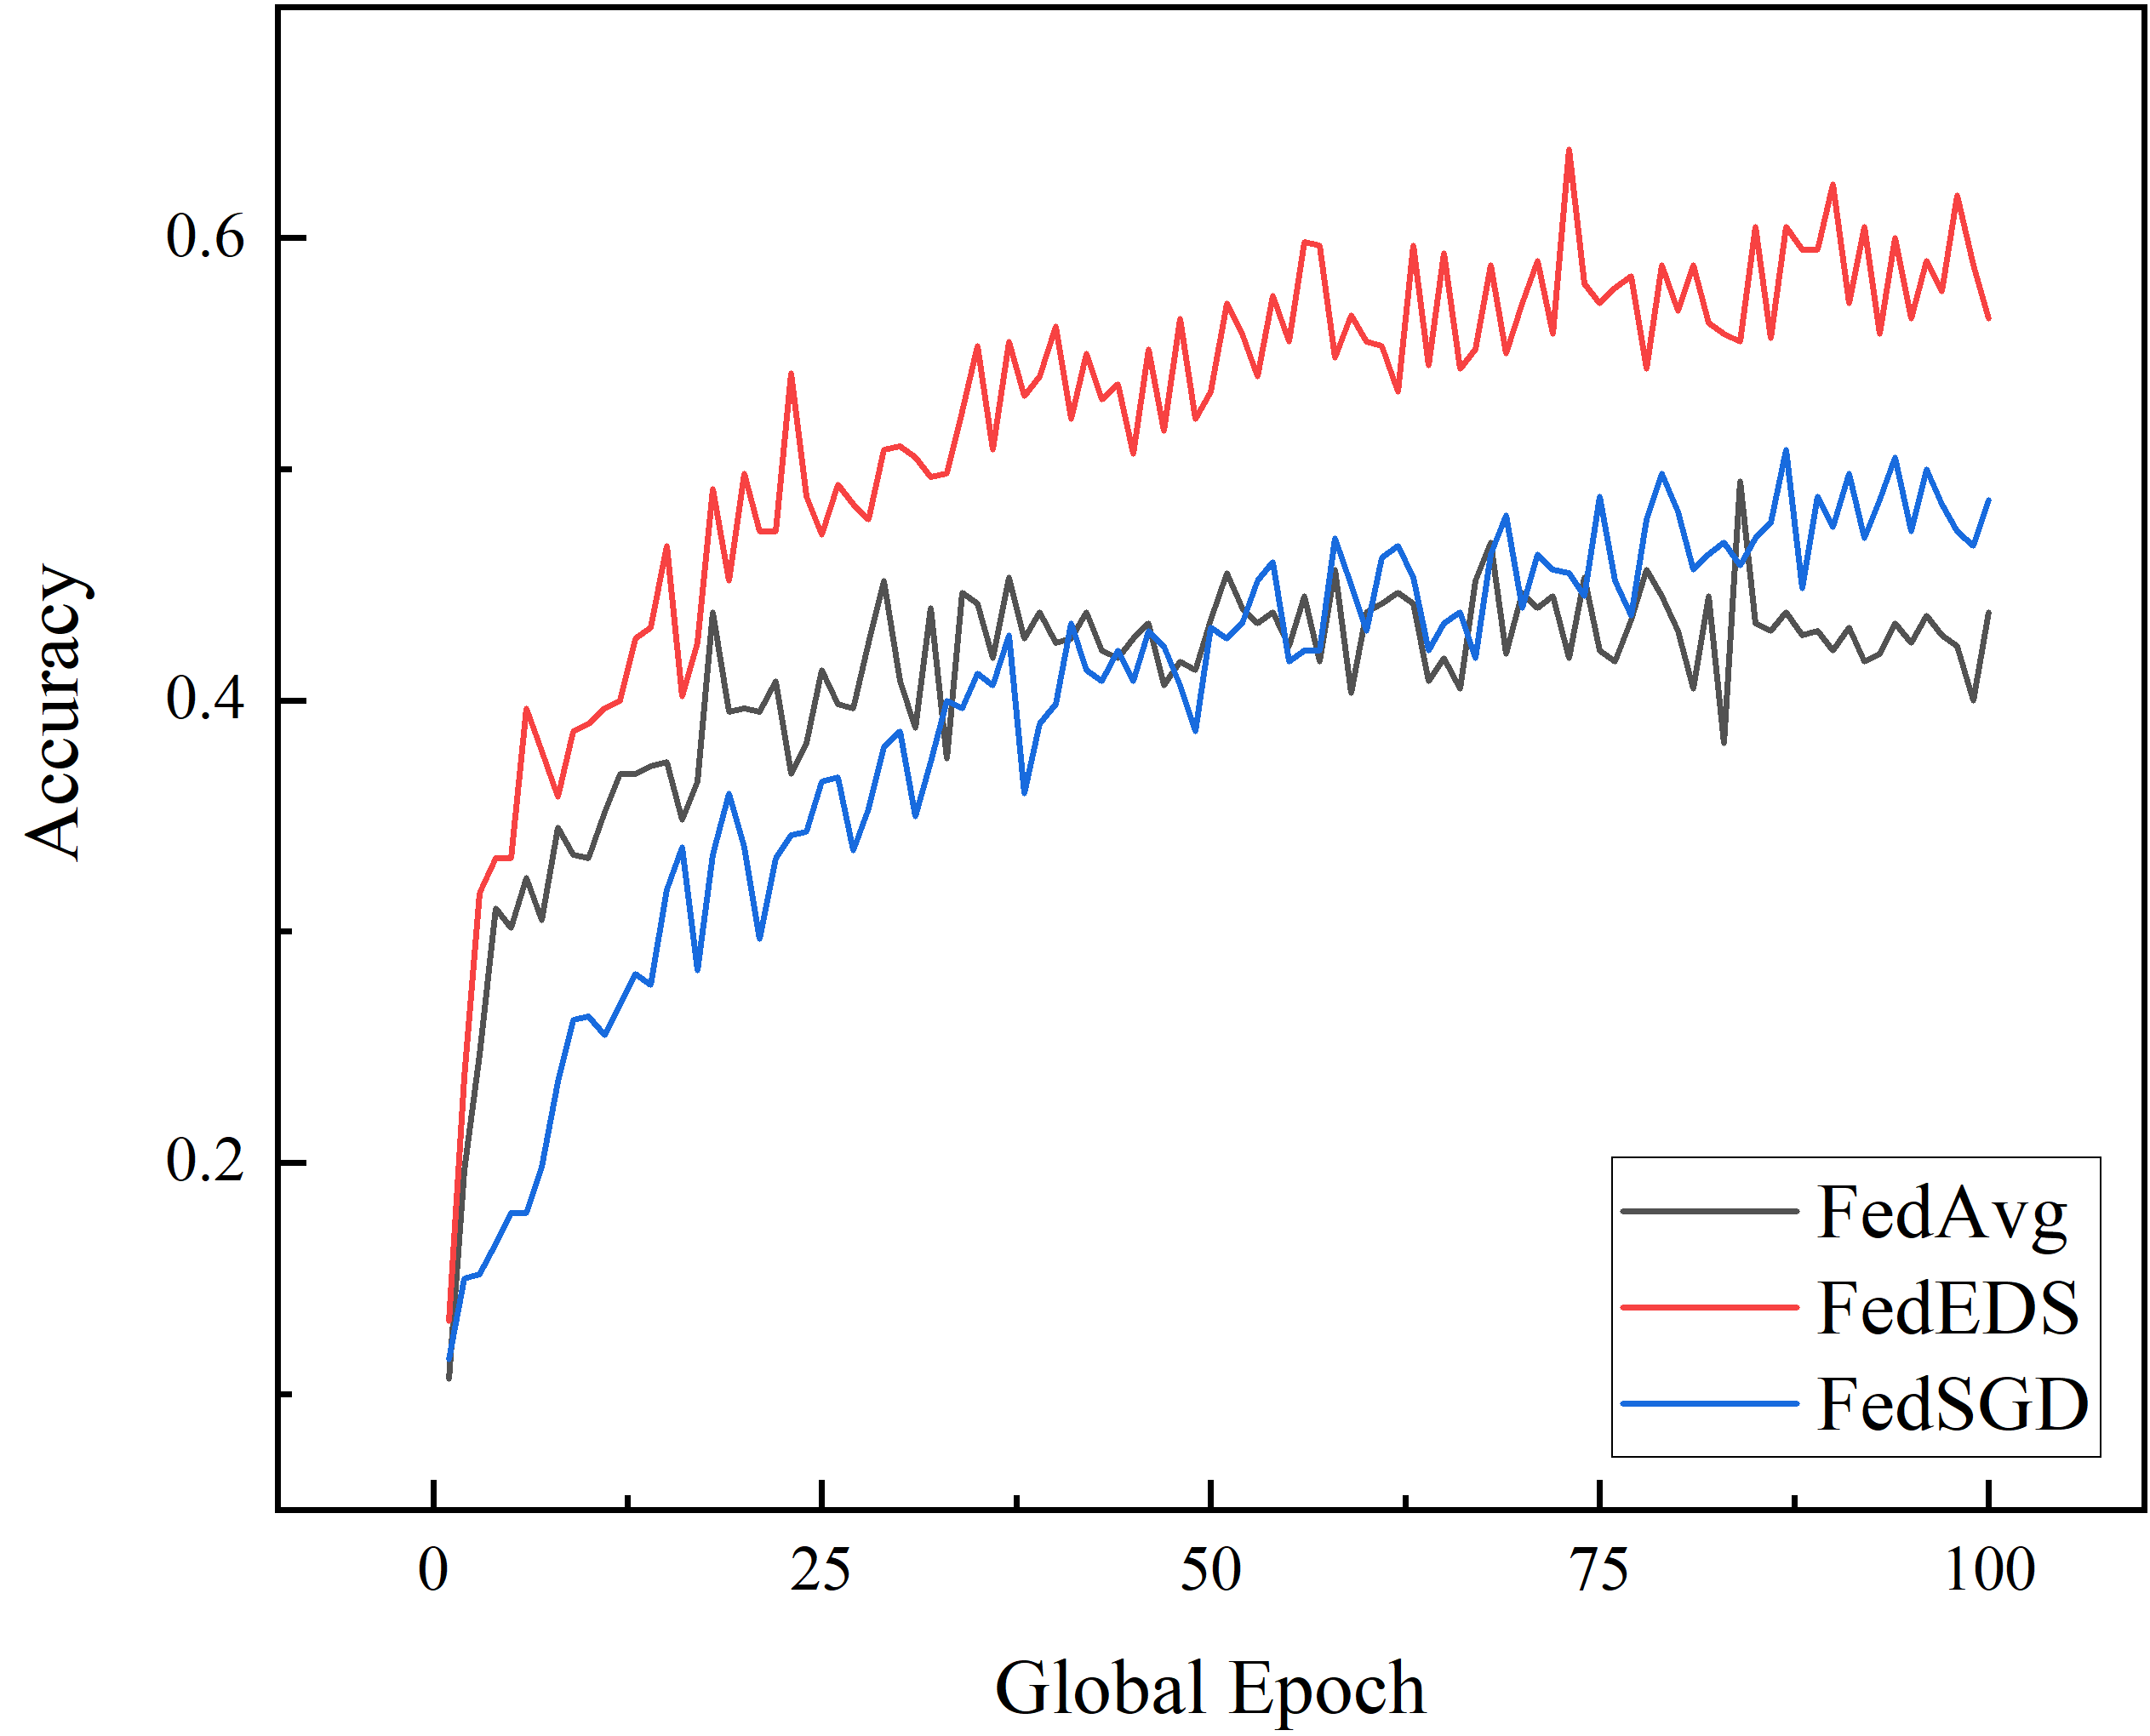
\includegraphics[width=0.33\textwidth]{CIFAR10_LeNet_PNG.png}}%\hspace{0.01in}
  % \vspace{-0.1in}
  \caption{Global Accuracy of FedAvg, FedSGD and FedEDS}\label{fig:profit-kn-2}\vspace{-0.15in}
  \end{minipage}%
  % \vspace{-0.05in}
  \end{figure*}
  \begin{figure*}[!t]
    %\subfigure[pic1.]{
    % \begin{minipage}[t]{0.25\linewidth}
    % \centering
    % %\subfigure[\label{revenue-regret-KN}Revenue and regret]{\includegraphics[width=0.99\textwidth]{reven_regret_kn.eps}}%\hspace{0.01in}
    % \includegraphics[width=0.99\textwidth]{EM_PNG.png}
    % \vspace{-0.2in}
    % \caption{}}\label{fig:revenue-regret-CMAB-KN-2}\vspace{-0.15in}
    % \end{minipage}%
    % %}%
    \begin{minipage}[t]{0.75\linewidth}
    \centering
    \subfigure[\label{fig:1profit_c_kn-2}MNINST with AlexNet]{\includegraphics[width=0.33\textwidth]{MNIST_GROUP_AlexNet_PNG.png}}%\hspace{0.01in}
    \subfigure[\label{fig:1profit_p_kn-2}MNINST with LeNet-5]{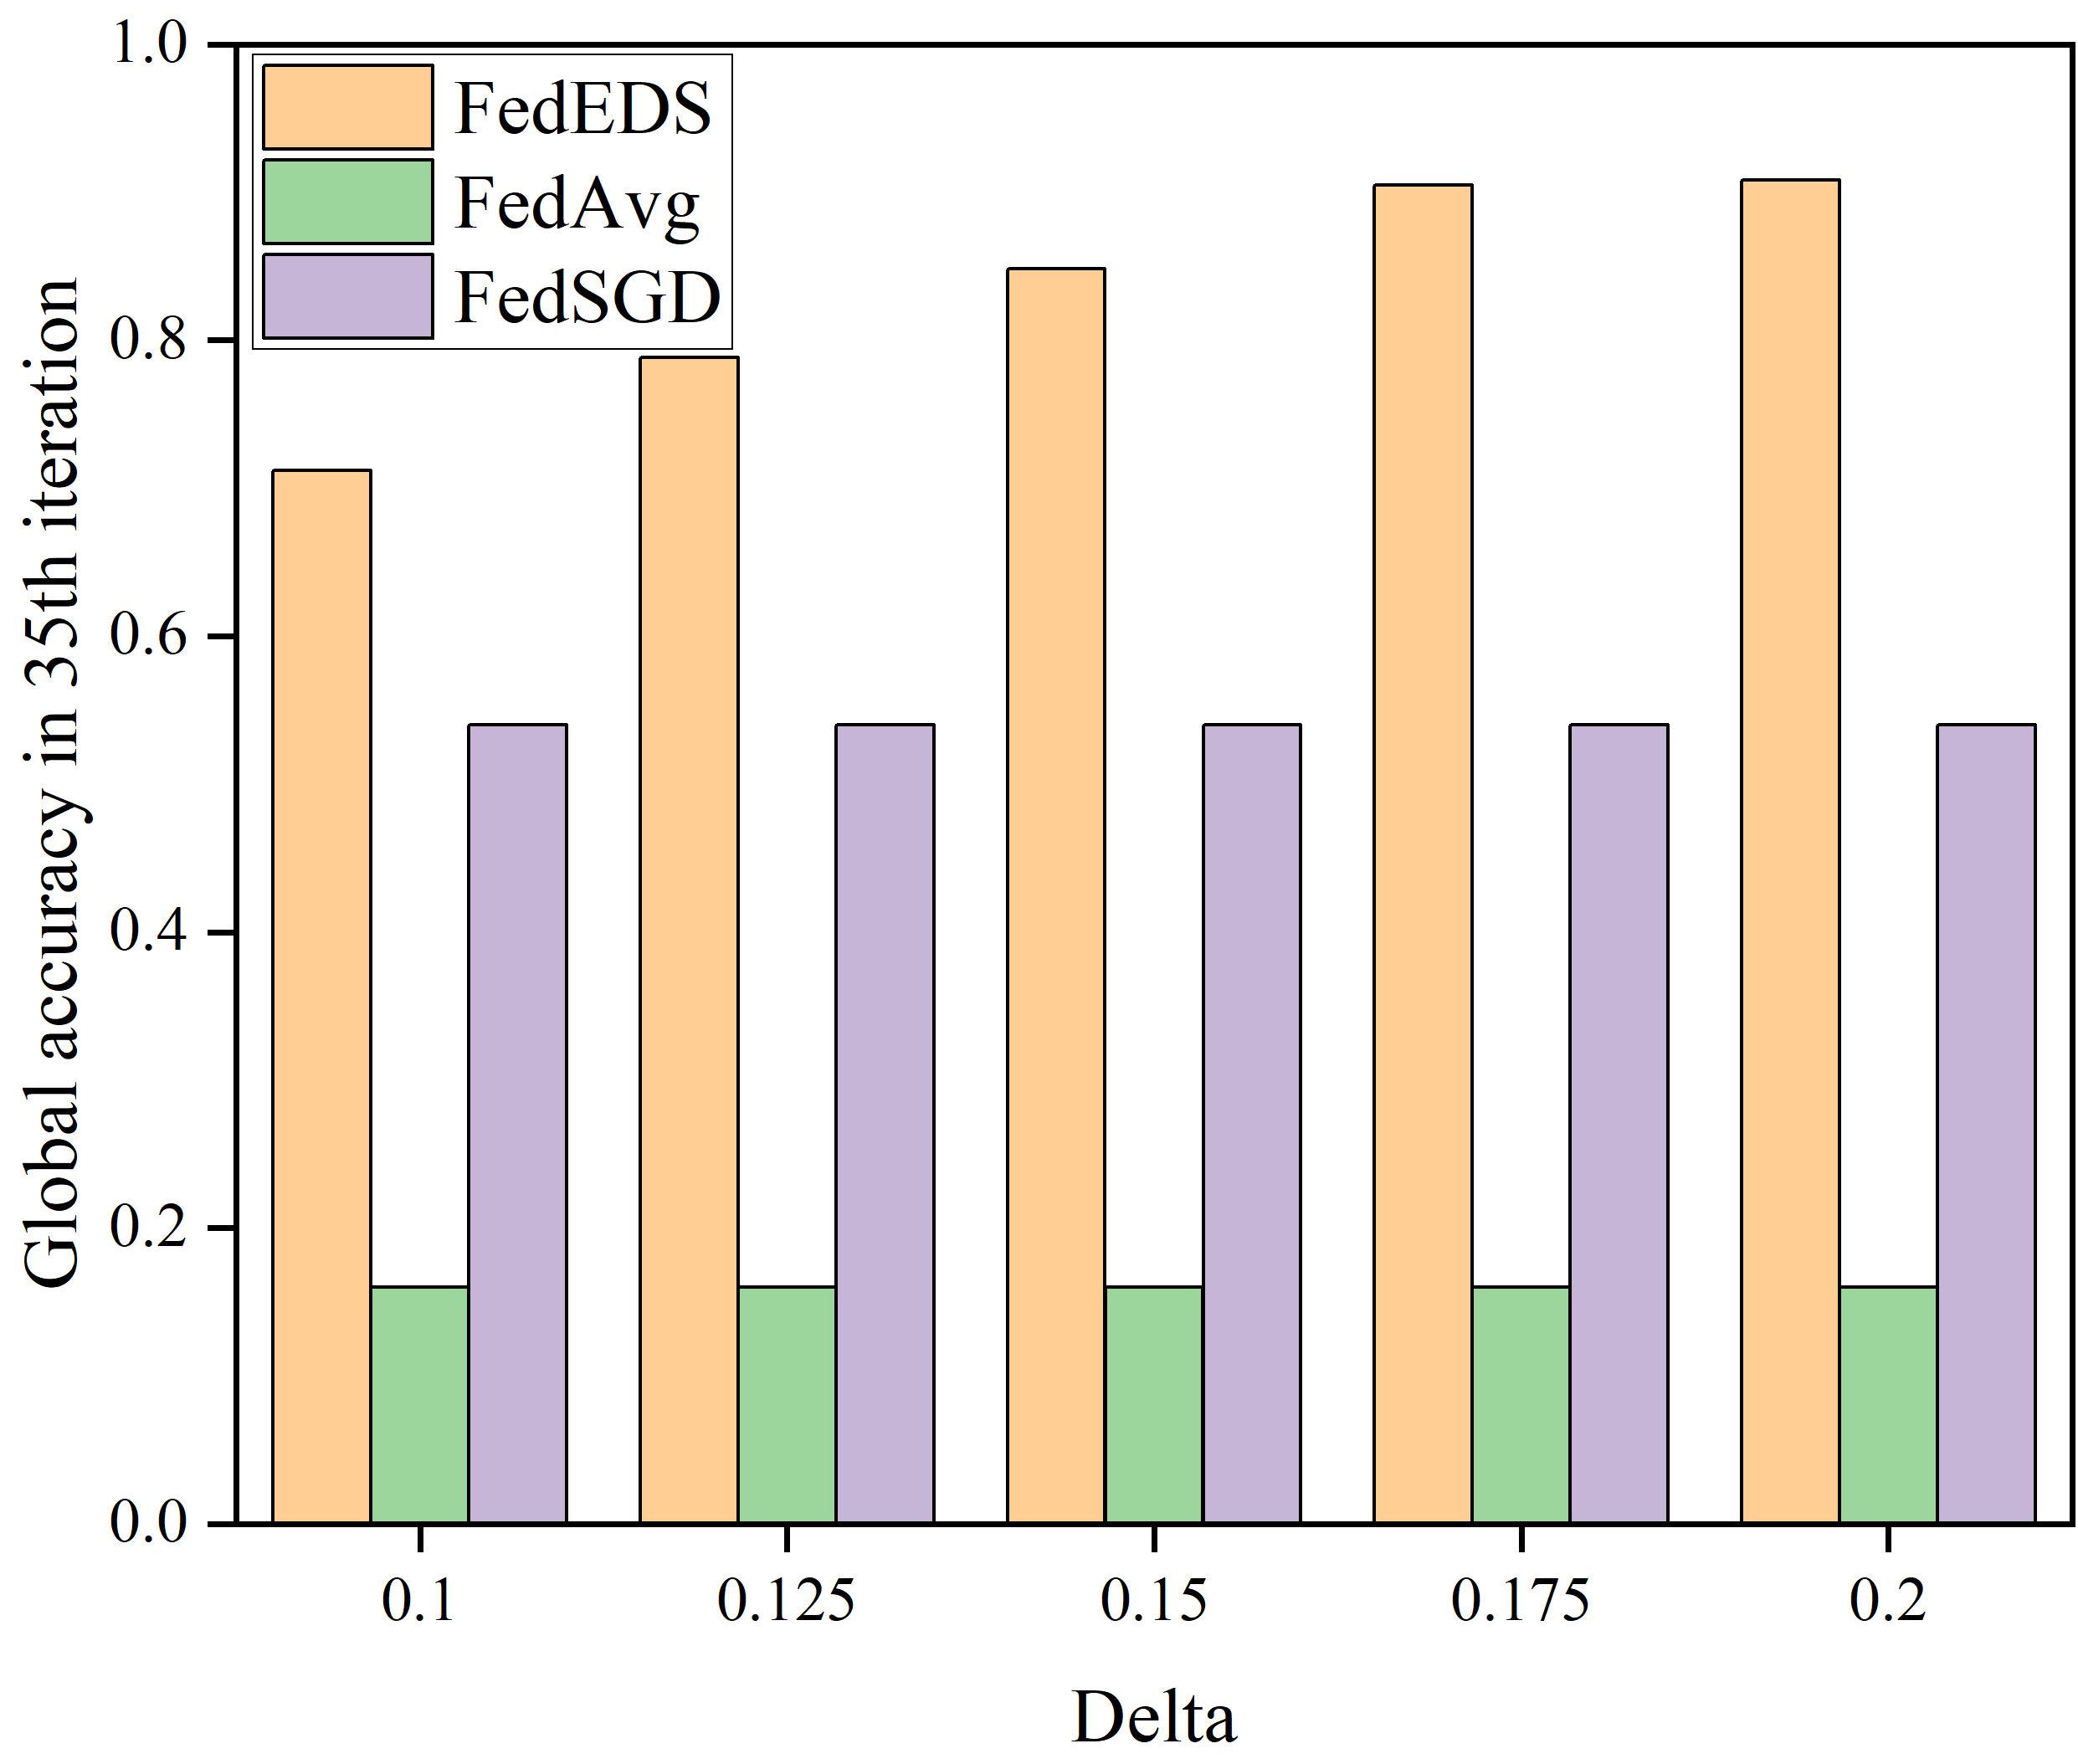
\includegraphics[width=0.33\textwidth]{MNIST_GROUP_LeNet_PNG.png}}%\vspace{-0.01in}
    \subfigure[\label{fig:1profit_s_kn-2}CIFAR-10 with AlexNet]{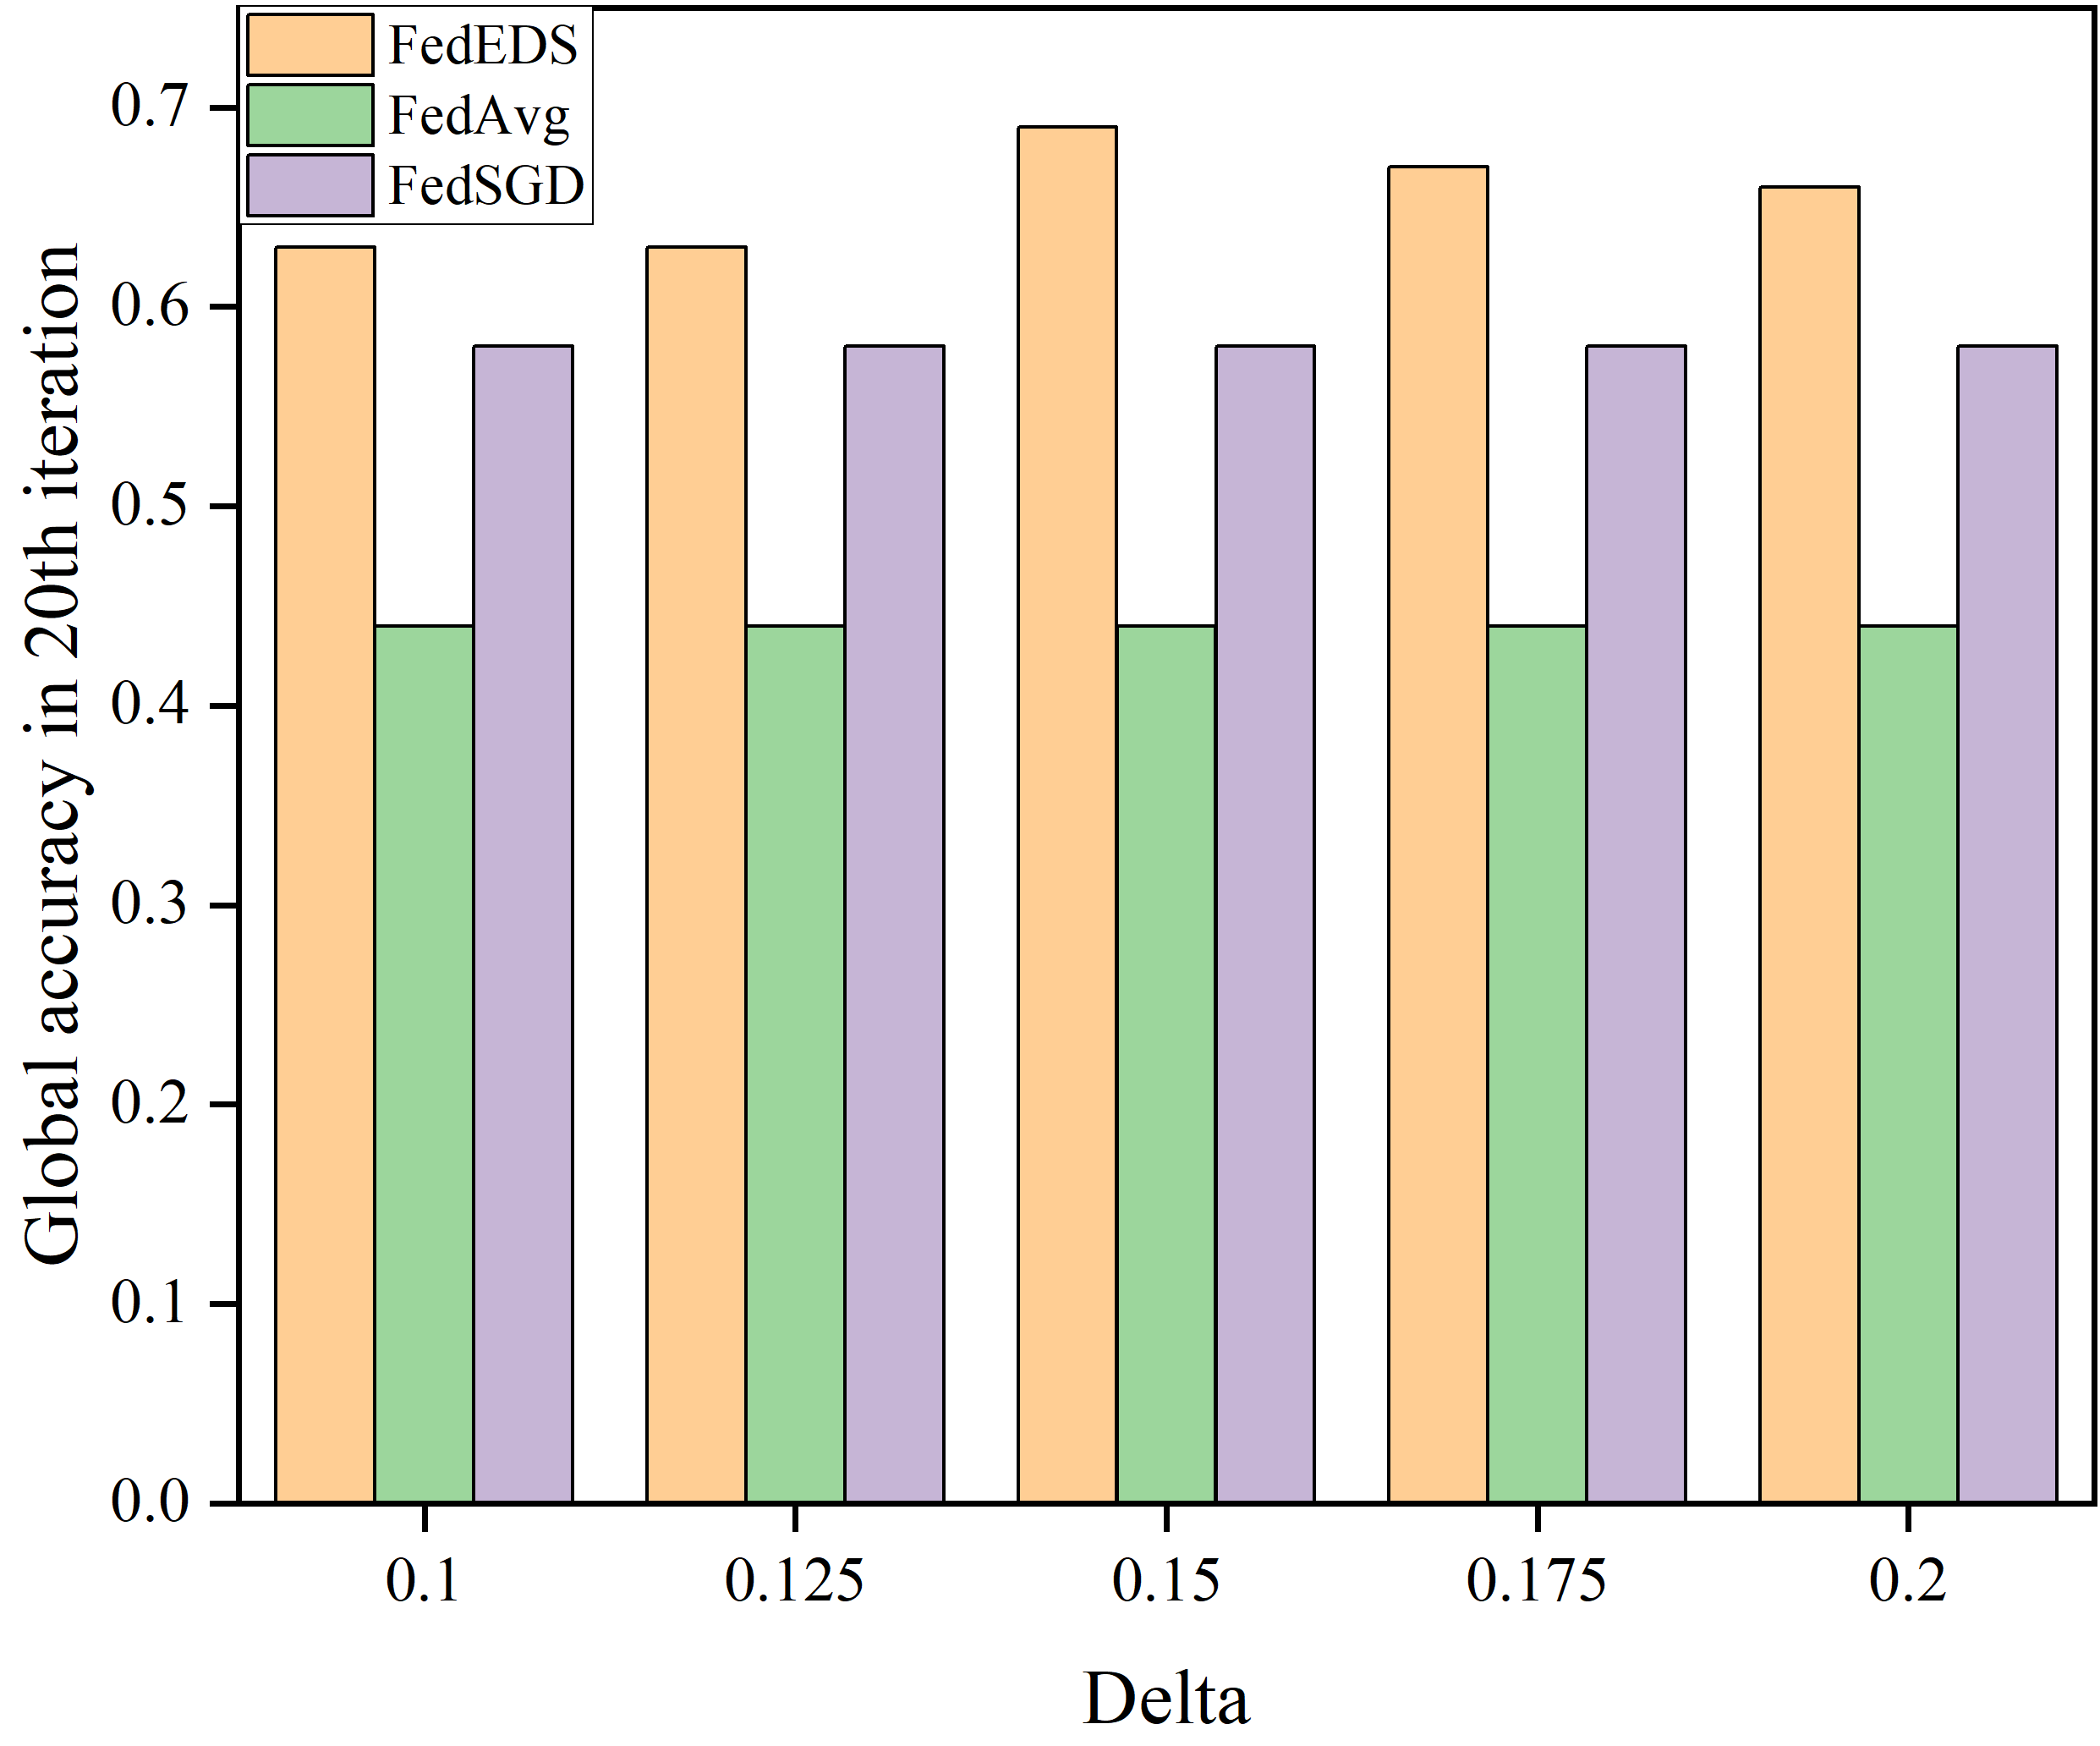
\includegraphics[width=0.33\textwidth]{CIFAR_GROUP_AlexNet_PNG.png}}%\vspace{-0.01in}
    \subfigure[\label{fig:1profit_c_kn-3}CIFAR-10 with LeNet-5]{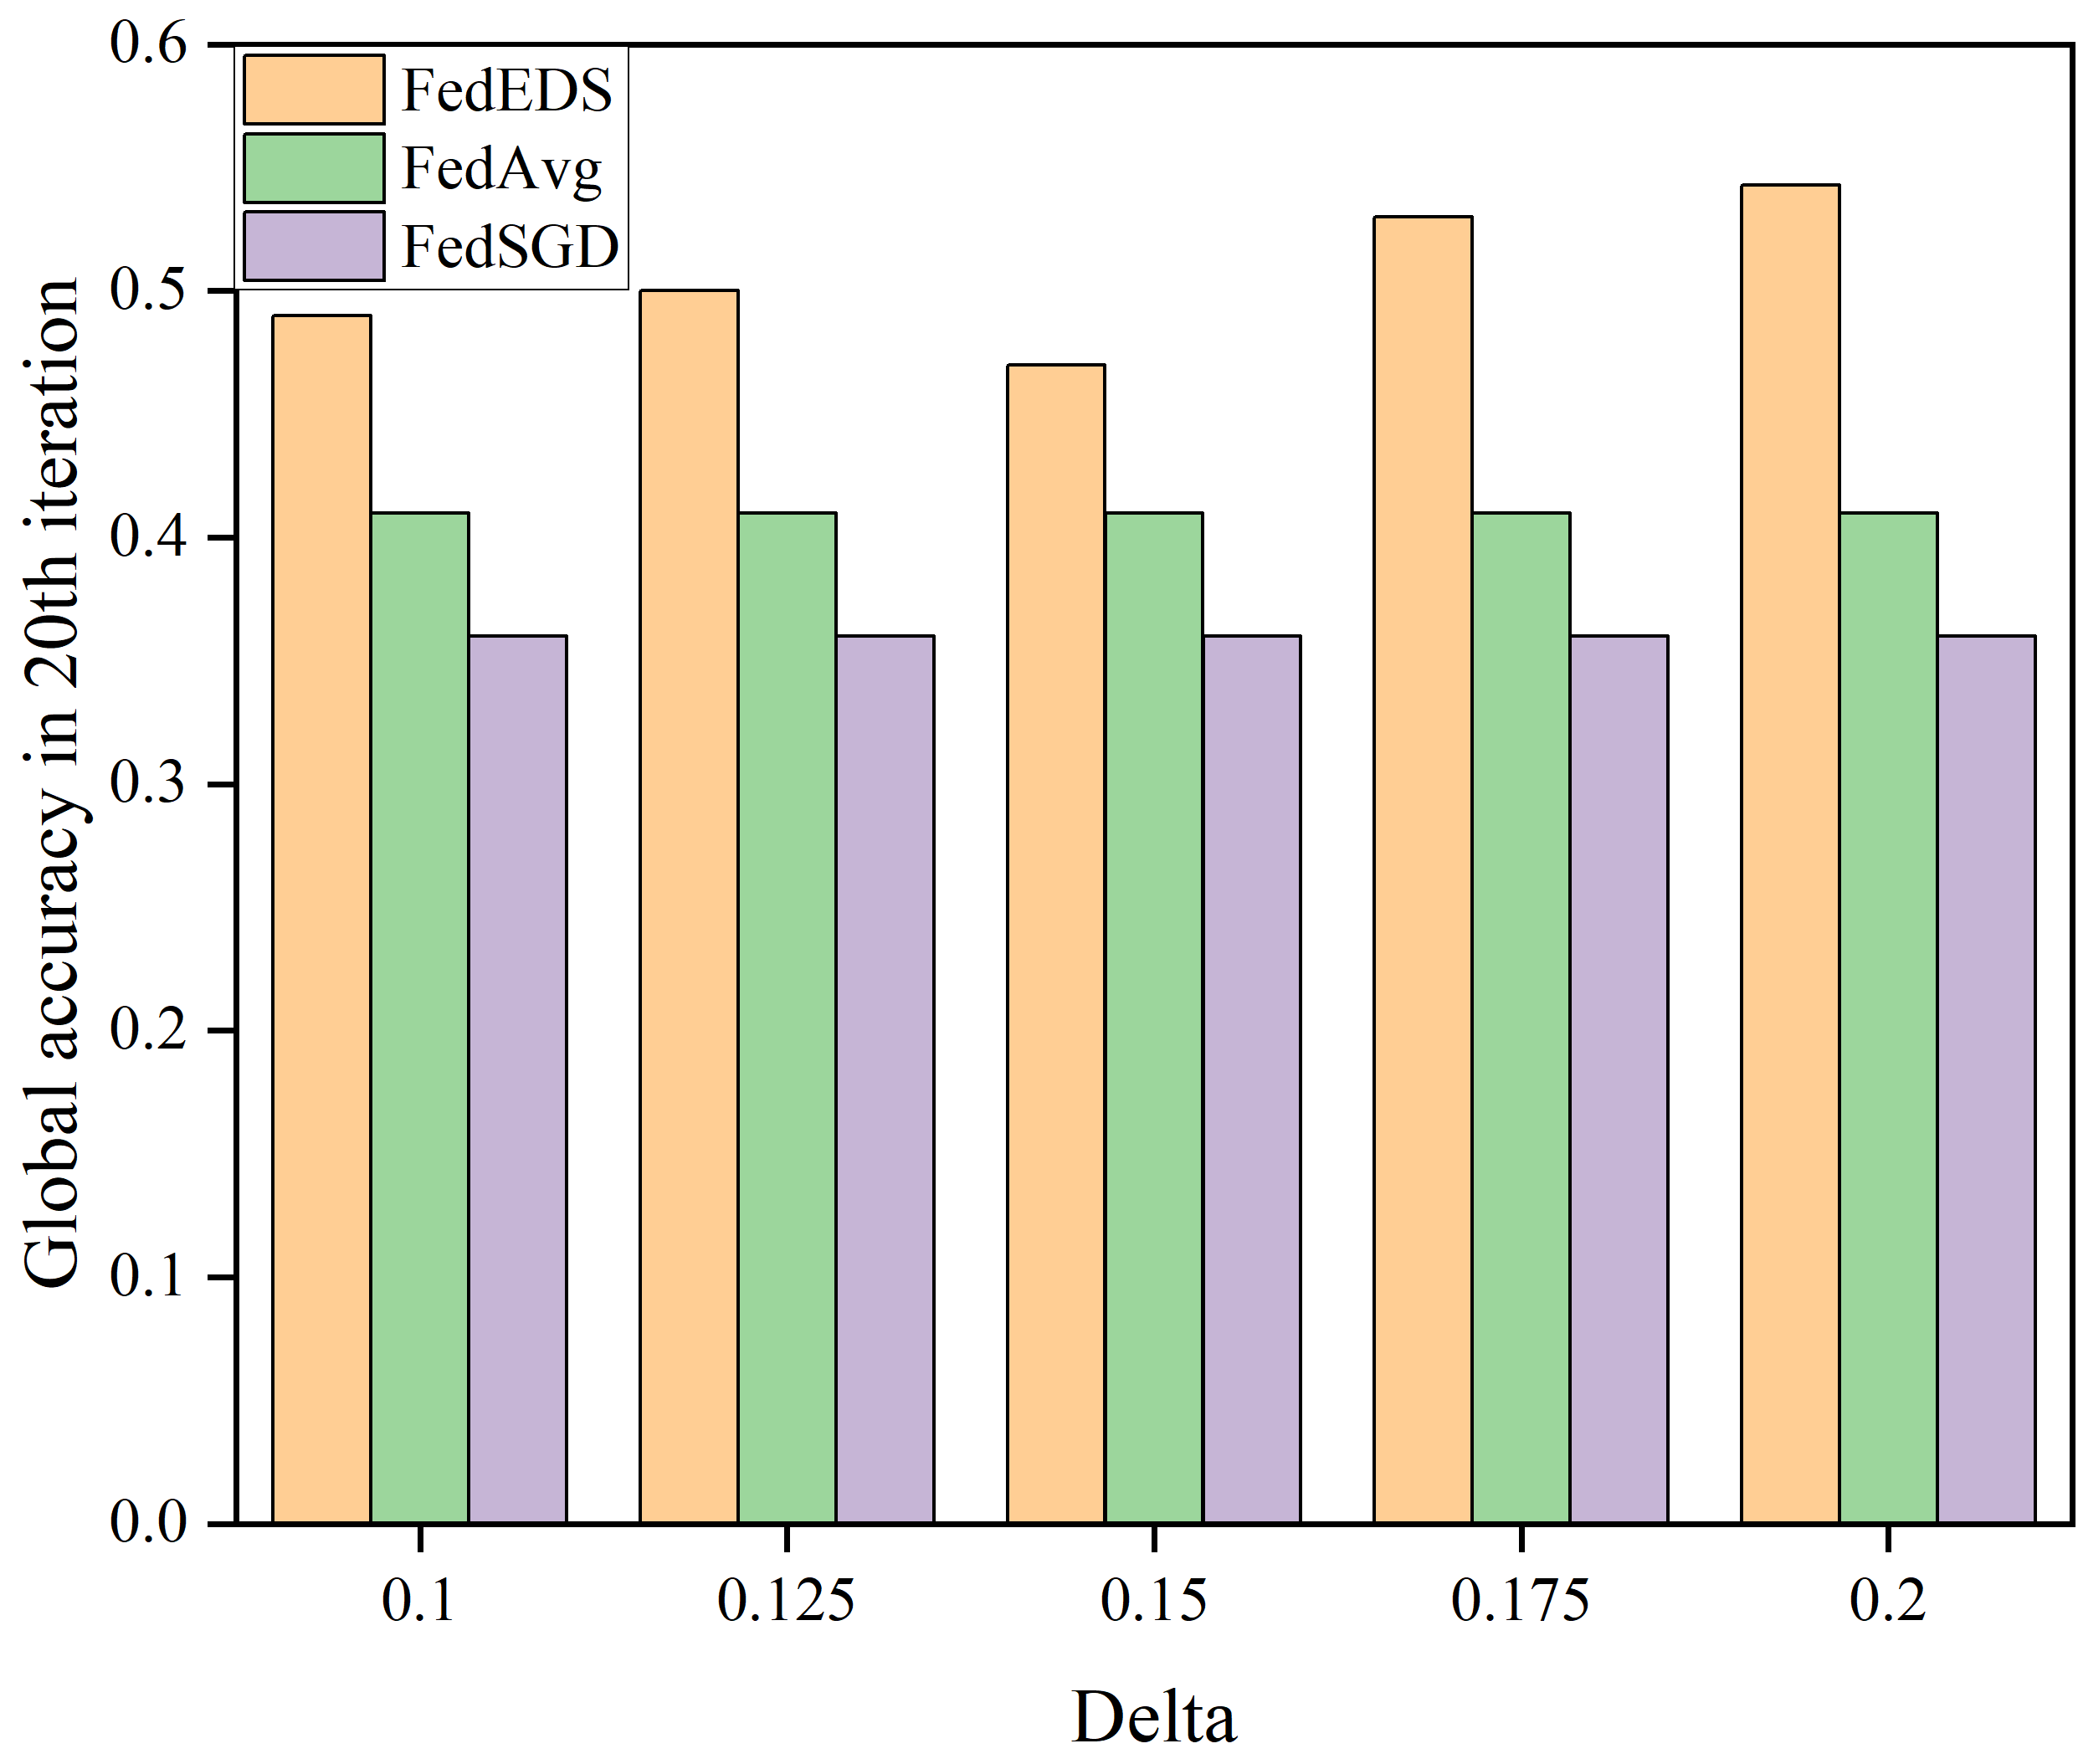
\includegraphics[width=0.33\textwidth]{CIFAR_GROUP_LeNet_PNG.png}}%\hspace{0.01in}
    % \vspace{-0.1in}
    \caption{Global Accuracy of FedAvg, FedSGD and FedEDS in Different $\delta_s$}\label{fig:profit-kn-2}\vspace{-0.15in}
    \end{minipage}%
    % \vspace{-0.05in}
    \end{figure*}
\begin{table}
    \caption{Estimation Results}
    \begin{tabular}{|l|l|l|l|}
    \hline
    \multicolumn{1}{|c|}{\textbf{Epoch}} & \multicolumn{1}{c|}{\textbf{Mu}} & \multicolumn{1}{c|}{\textbf{Sigma}} & \multicolumn{1}{c|}{\textbf{Alpha}} \\ \hline
    \textbf{Standard}                    & (2.1,1.63,1.74)                  & (0.001,0.062,0.086)                 & (0.2,0.57,0.23)                     \\ \hline
    \textbf{1}                           & (1.51, 1.77, 1.80)               & (0.987 1.407 1.11)                  & (0.01,0.6,0.39)                     \\ \hline
    \textbf{5}                           & (1.86, 1.78, 1.78)               & (0.201, 0.177, 0.178)               & (0.0,0.54,0.45)                     \\ \hline
    \textbf{10}                          & (1.91, 1.78, 1.78)               & (0.196,0.177, 0.179)                & (0.0,0.54,.045)                     \\ \hline
    \textbf{100}                         & (2.10, 1.67, 1.7)                & (0.001,0.083, 0.085)                & (0.2,0.49,0.30)                     \\ \hline
    \textbf{400}                         & (2.10, 1.65, 1.77)               & (0.001,0.072, 0.075)                & (0.2, 0.45, 0.34)                   \\ \hline
    \end{tabular}
    \end{table}
\subsubsection{Model Setting}
AlexNet\cite{krizhevsky2012imagenet} and LeNet-5\cite{lecun1998gradient} are the two kinds of improved convolutional neural networks 
(CNN). LeNet-5 is firstly proposed to solve the handwriting recognition problem,
it is composed of 7 layers, including 3 convolutional layers,
3 pooling layers, and 2 fully connected layers. Compared to LeNet-5, 
AlexNet enriches the CNN layers and adds LRN. With Relu function,
the AlexNet can converge faster and cost less than LeNet-5.
% \begin{figure}[t]
%     \centering
%     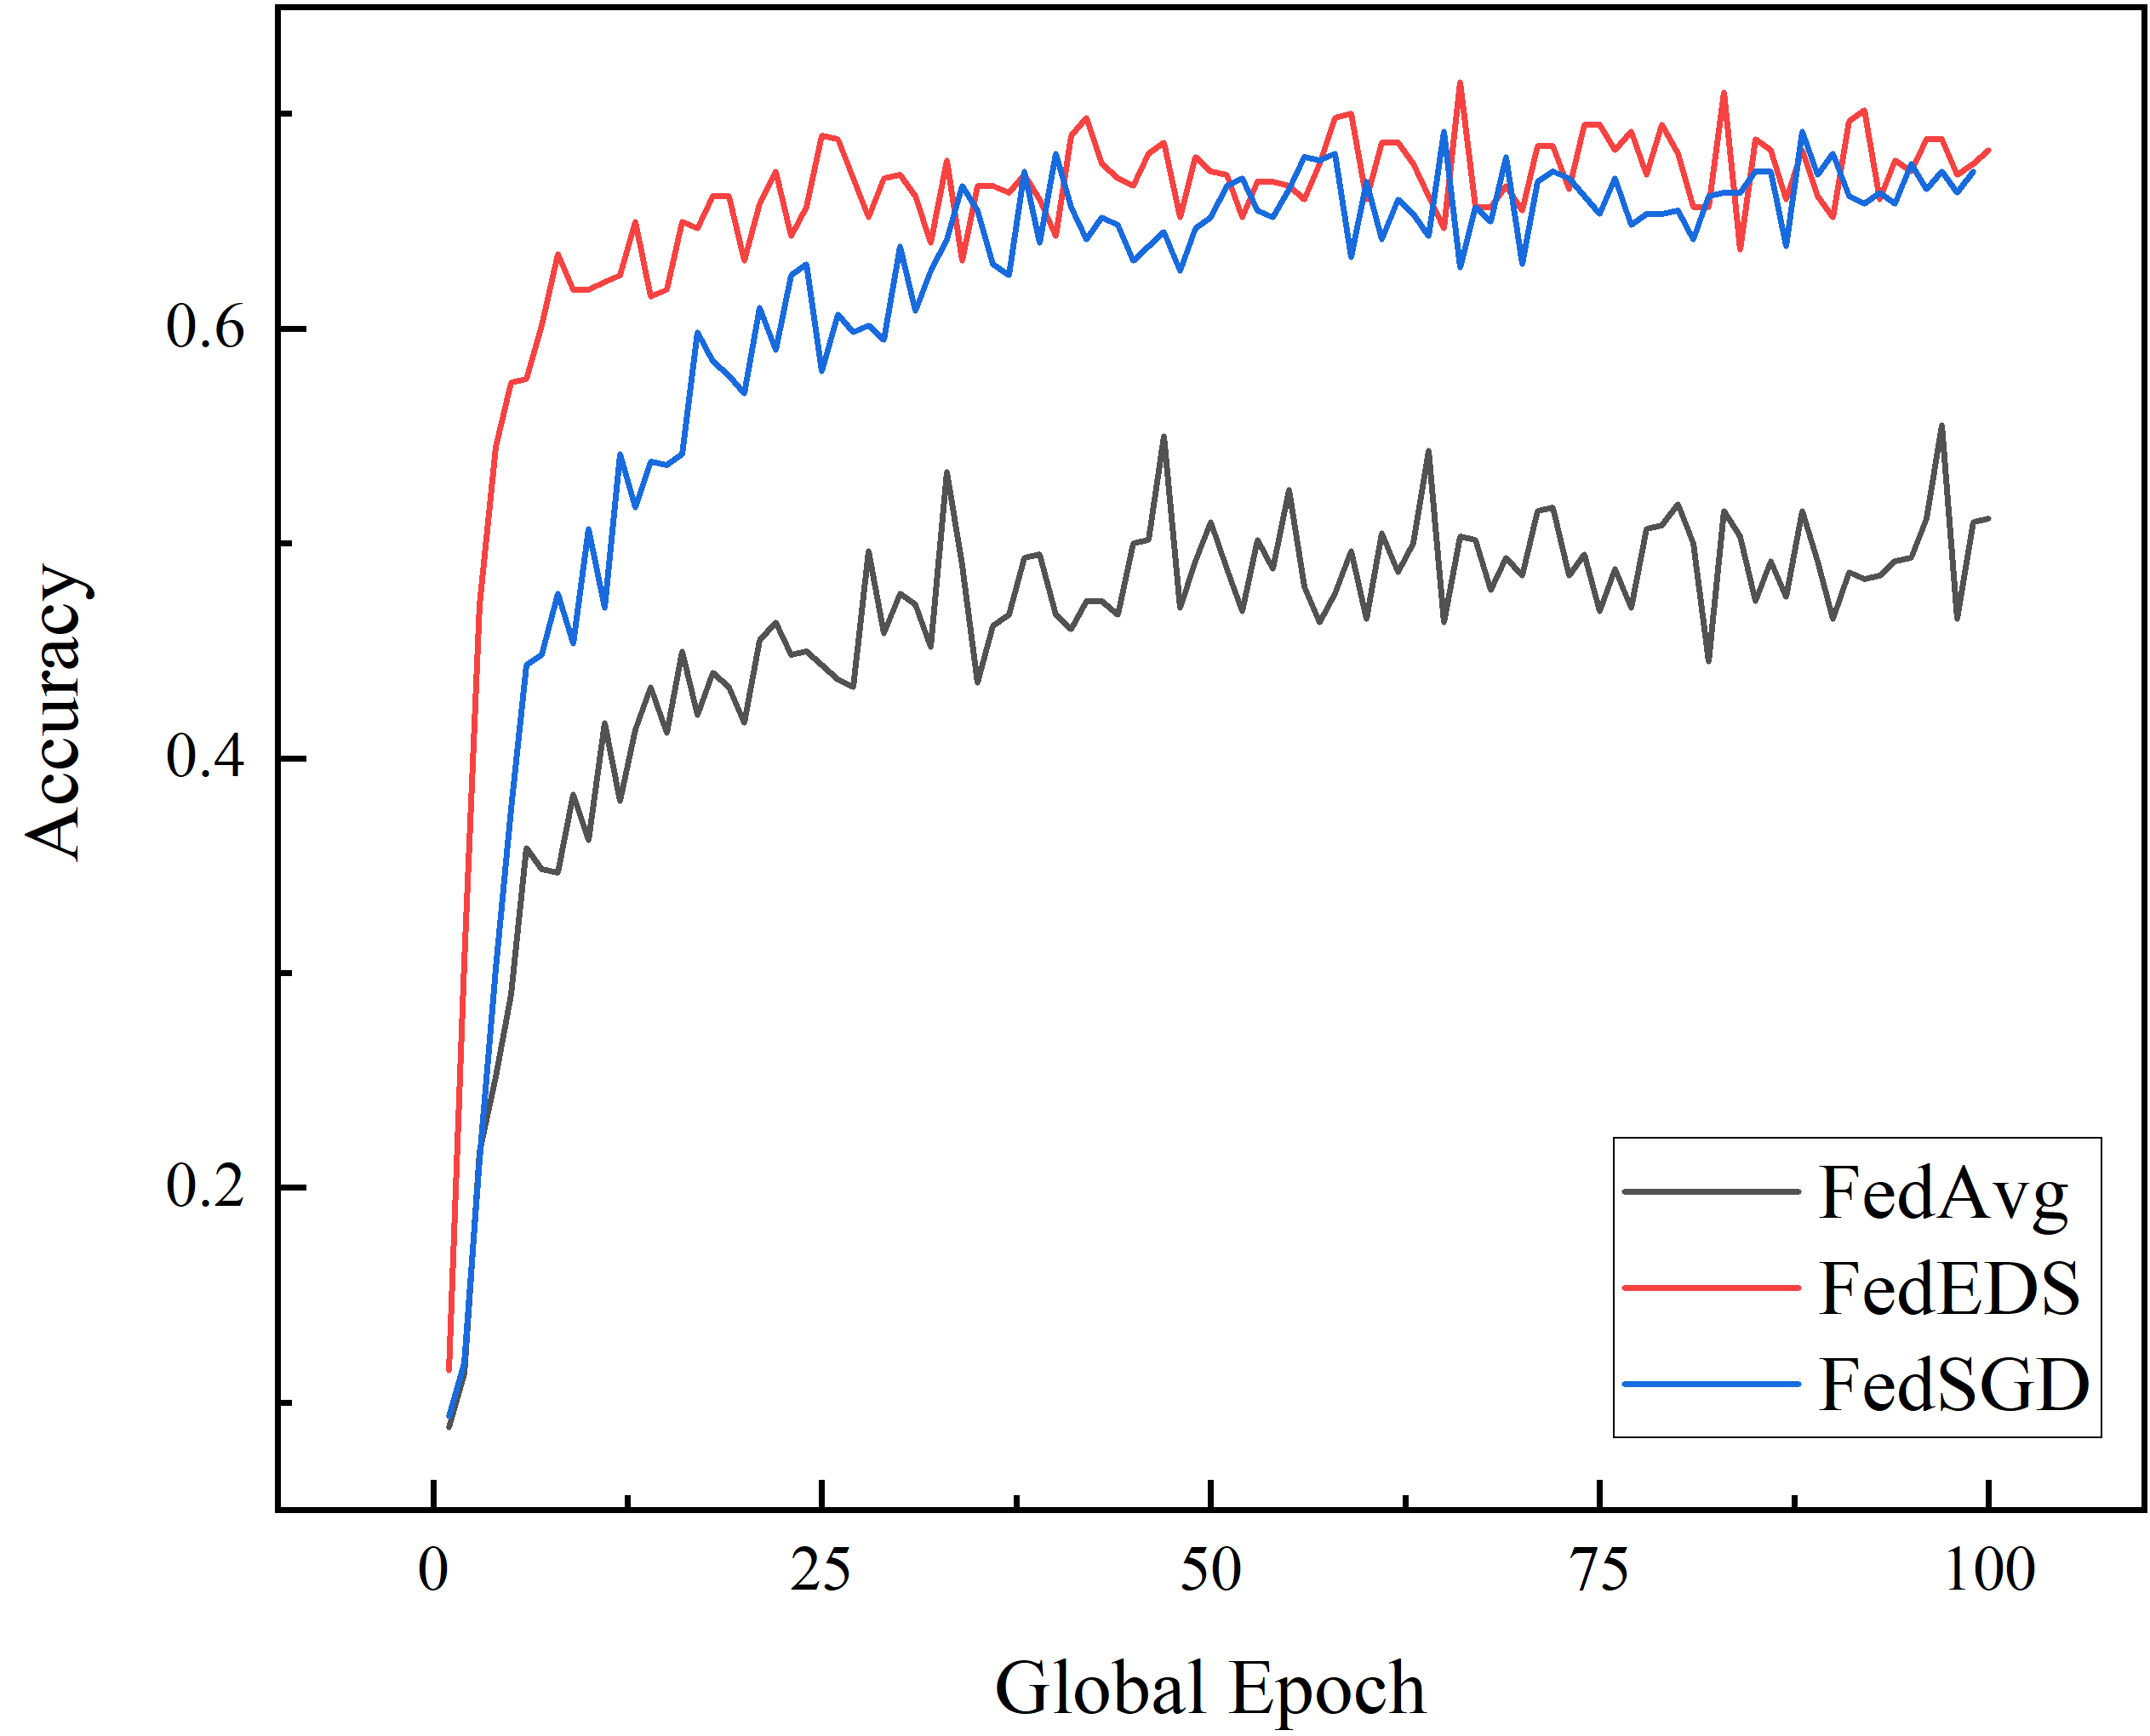
\includegraphics[height=3cm,width=4cm]{CIFAR10_AlexNet_PNG.png}
%     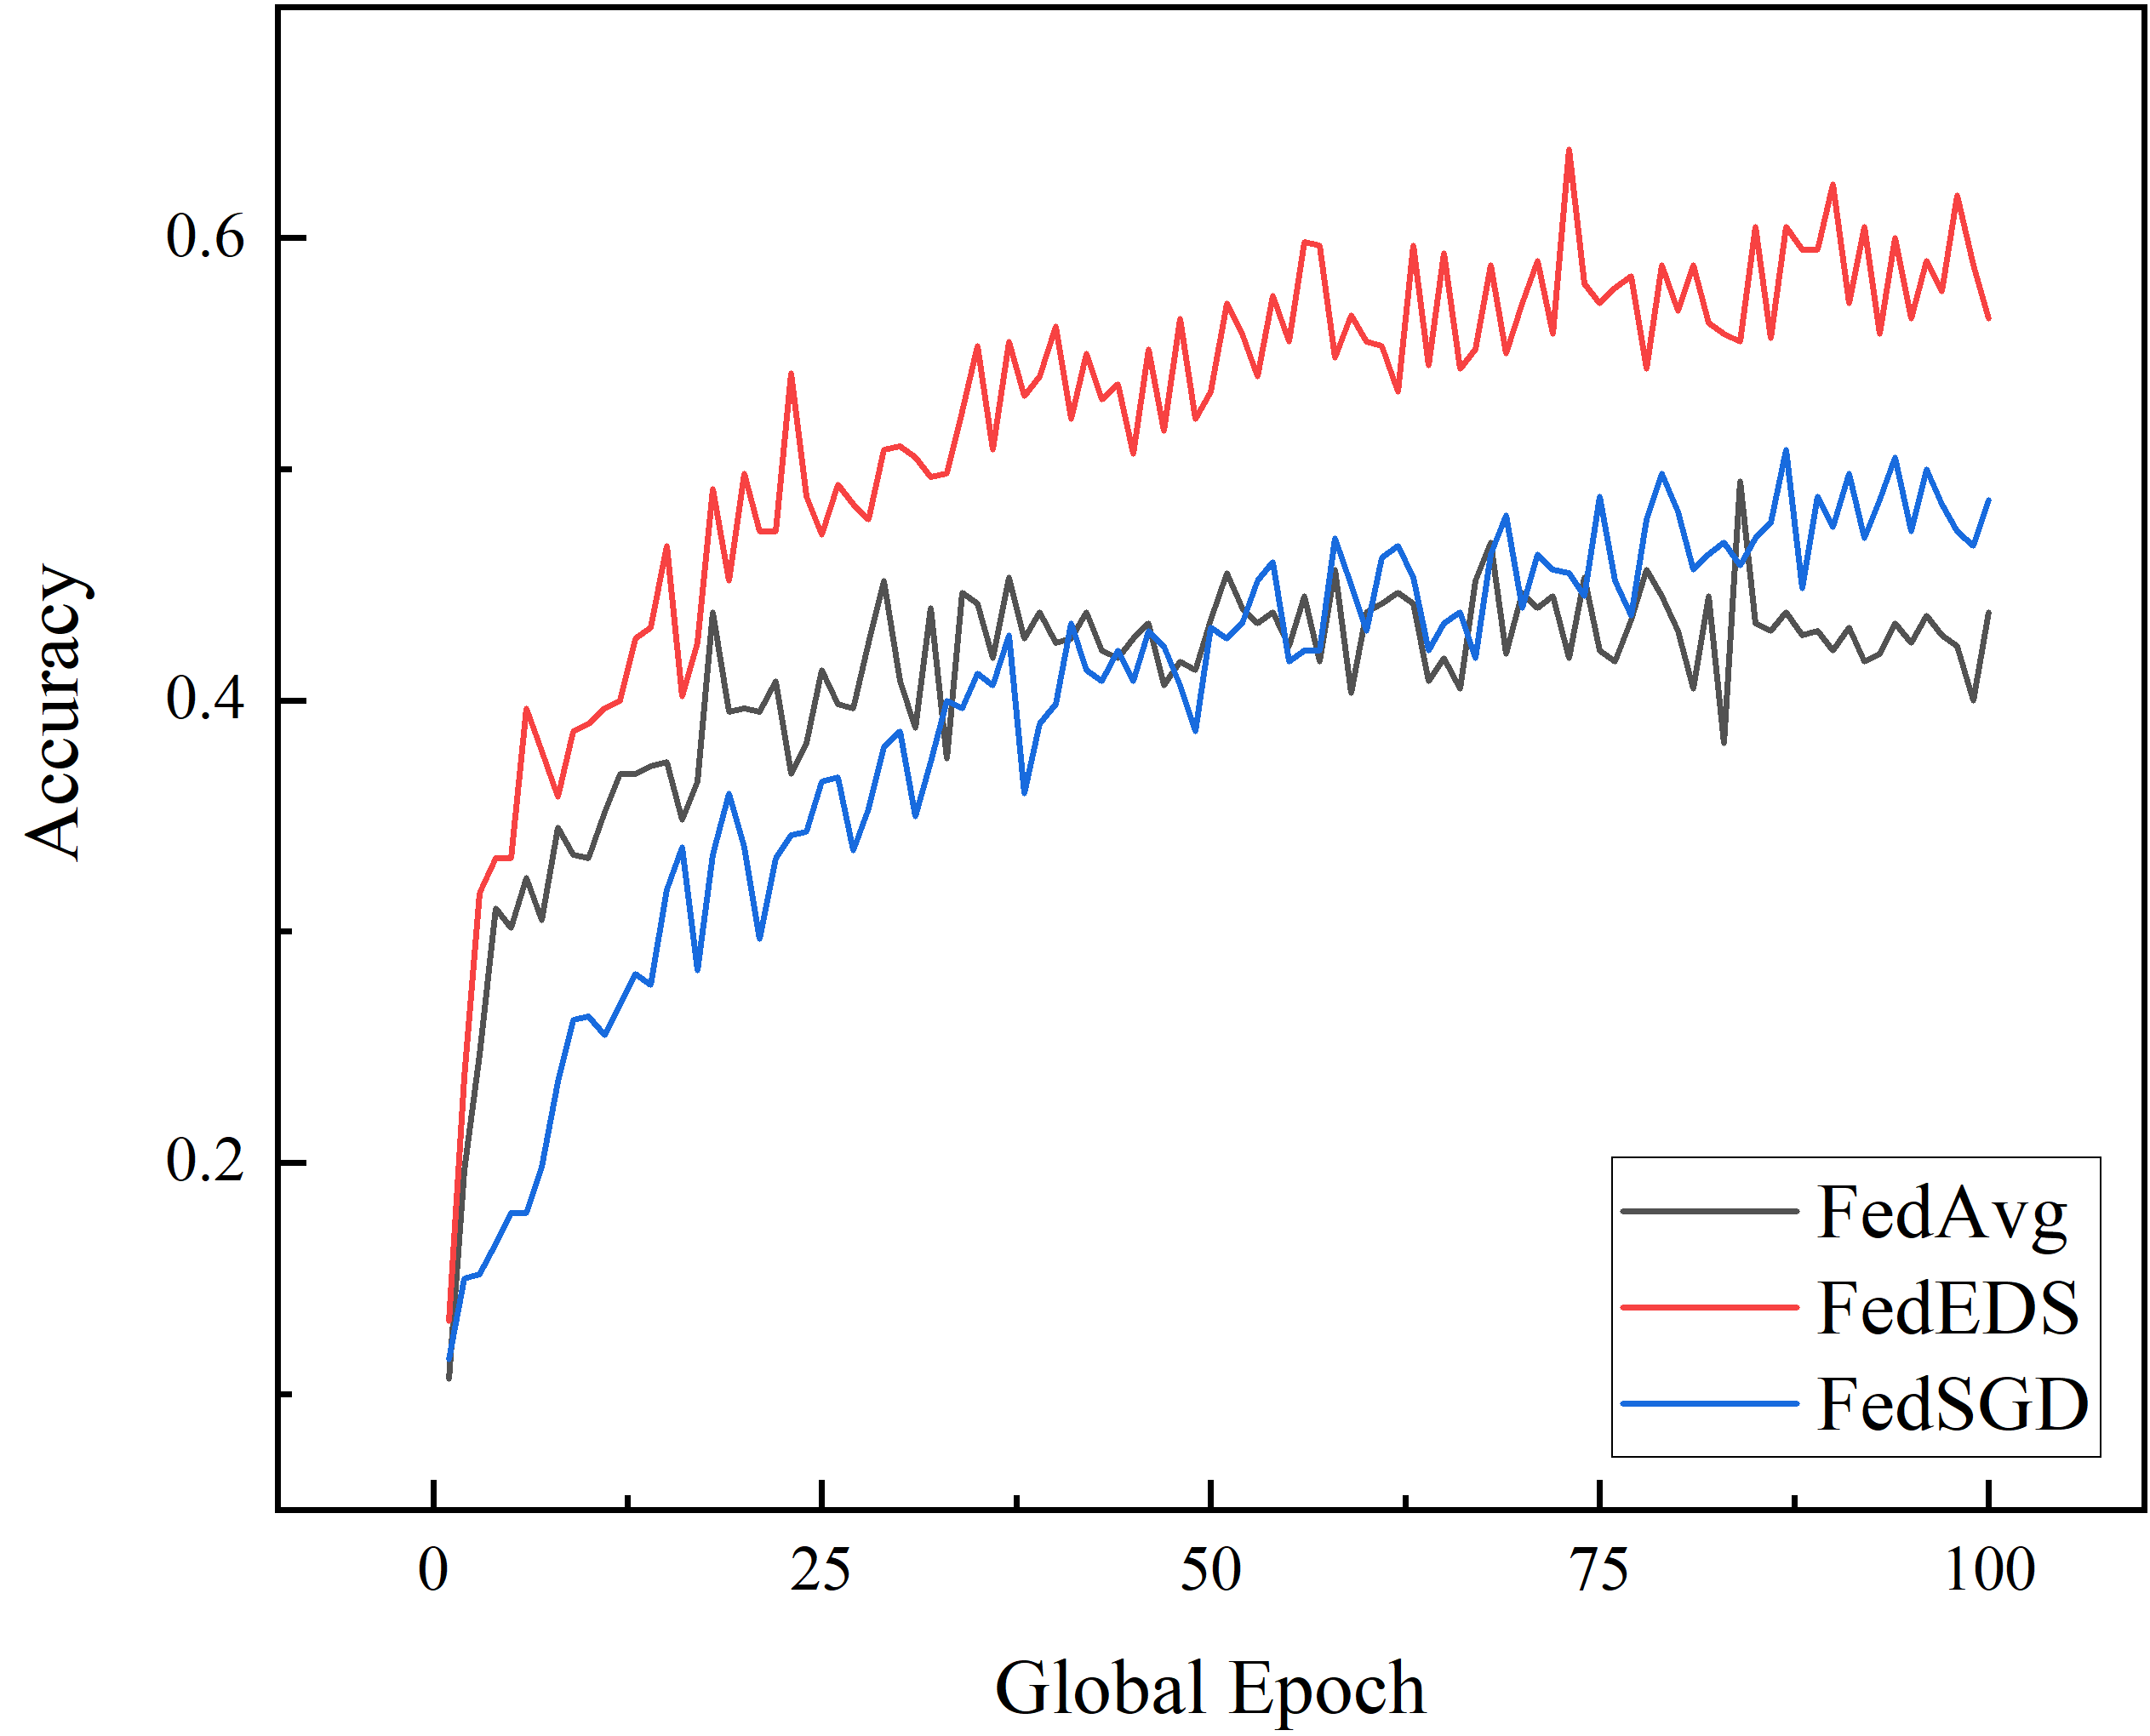
\includegraphics[height=3cm,width=4cm]{CIFAR10_LeNet_PNG.png}
%     \includegraphics[height=3cm,width=4cm]{MNIST_AlexNet_PNG.png}
%     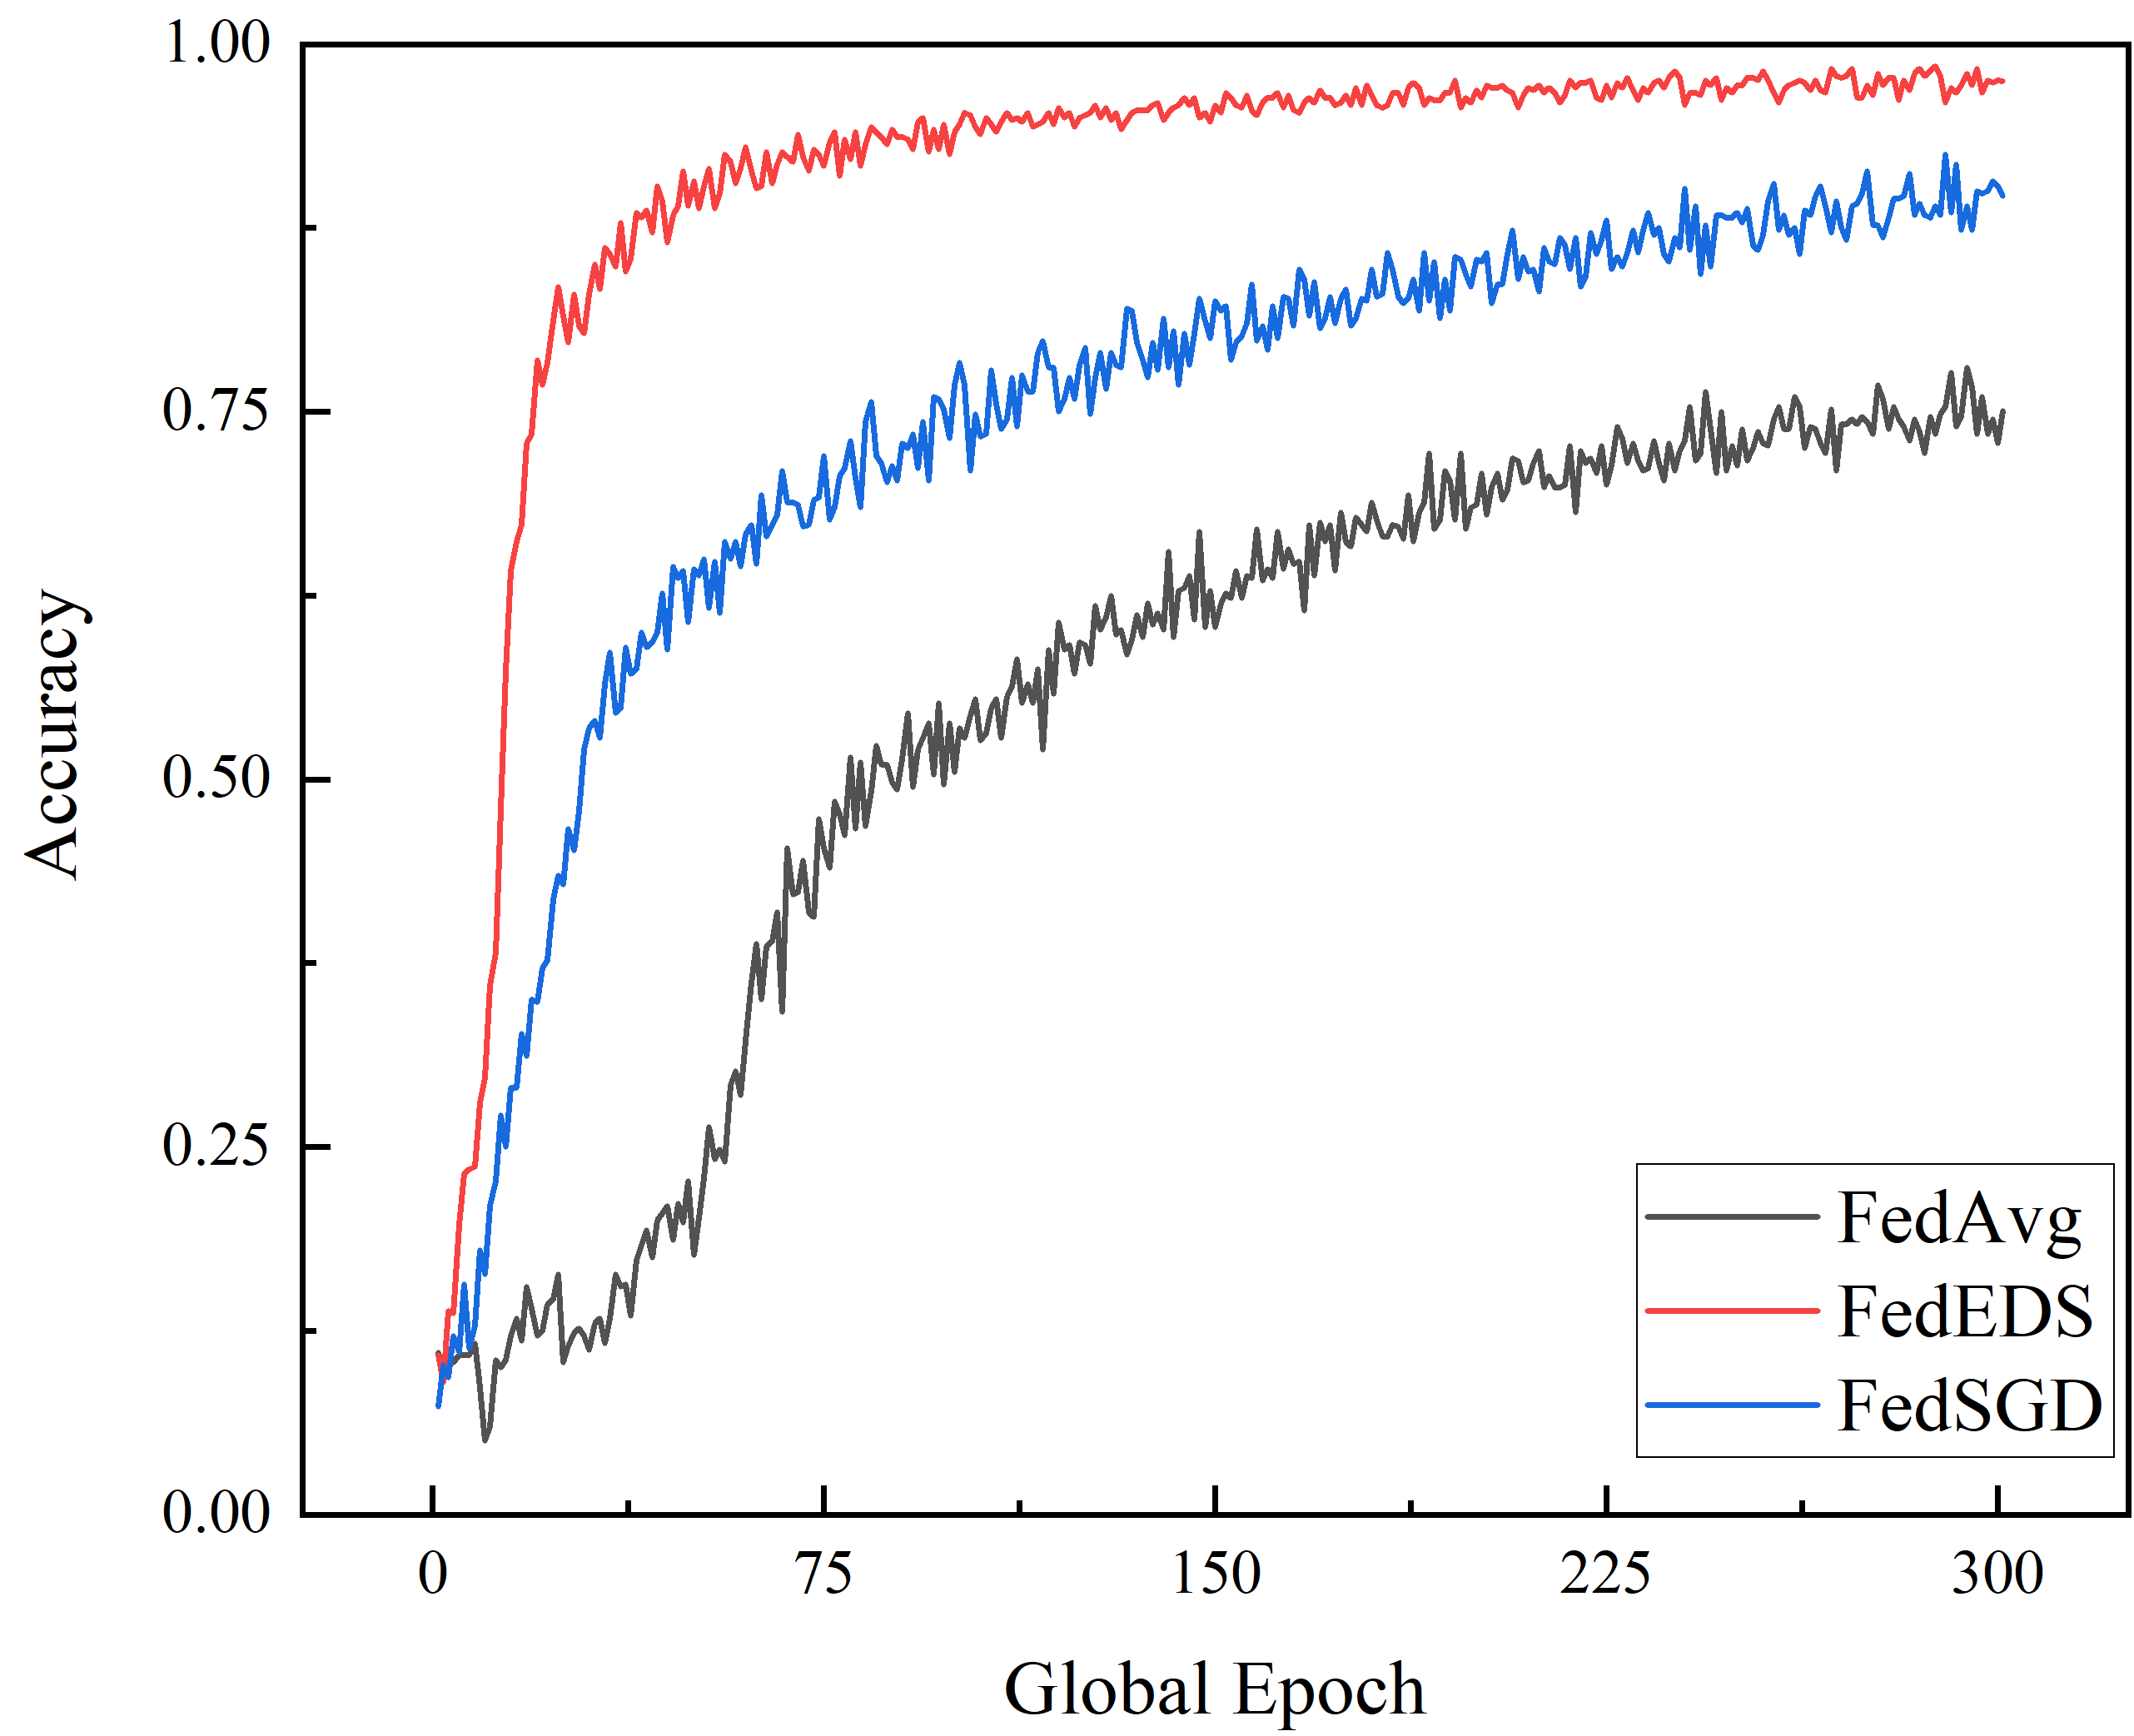
\includegraphics[height=3cm,width=4cm]{MNIST_LeNet_PNG.png}
%     \caption{Global Accuracy}
%     \label{CIFAR}
% \end{figure}
\subsubsection{Comparsion Setting}
We assume there exists at least one client which holds a lower quality, 
it typically can't achieve the preset threshold in the selection mechanism. 
Under this condition, we compare the performance of FedDCS, FedAvg, and FedSGD on 
the Non-IID data sets in different $\delta_s$. In addition, we measured the time consumption of
running algorithm programs in Intel SGX Enclave, which aims to prove the loss
is acceptable.

% Our selection mechanism works especially efficiently in real scenarios
% based on gauss model, in other situations, the performance of our 
% framework is no less than FedAvg. 
% \begin{figure}
%     \centering 
%     \includegraphics[height=3cm,width=4cm]{MNIST_GROUP_AlexNet_PNG.png}
%     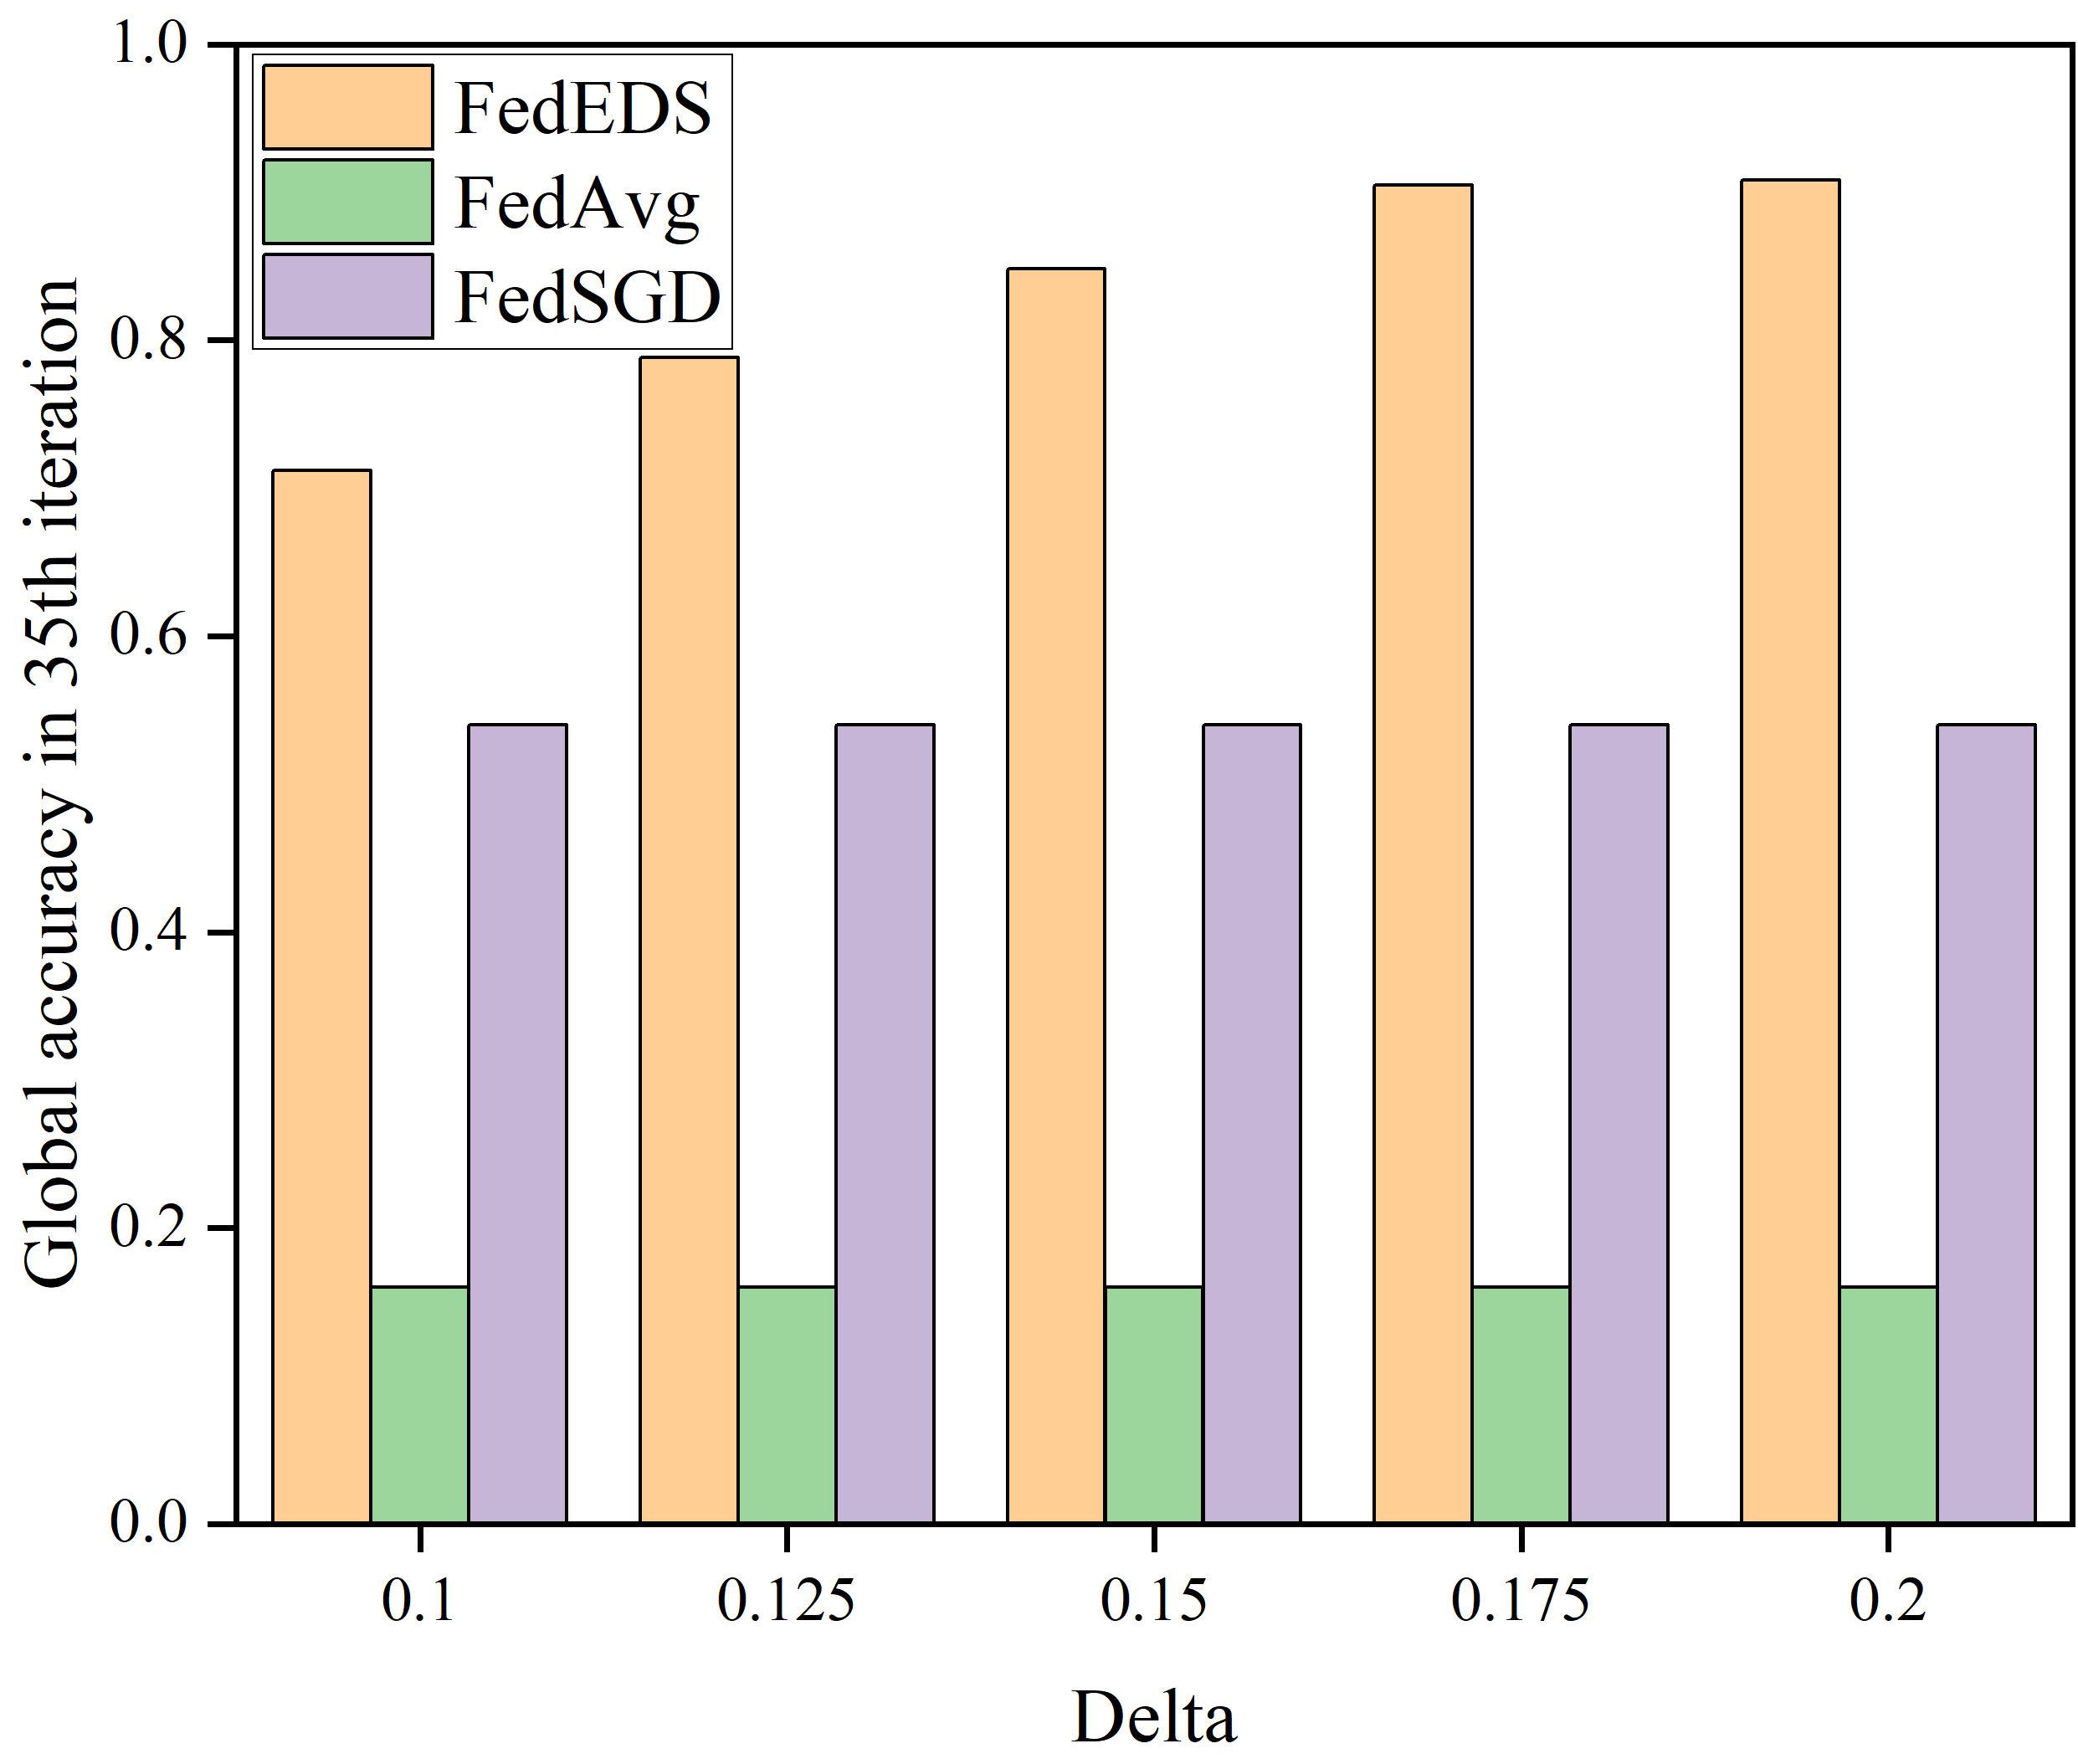
\includegraphics[height=3cm,width=4cm]{MNIST_GROUP_LeNet_PNG.png}
%     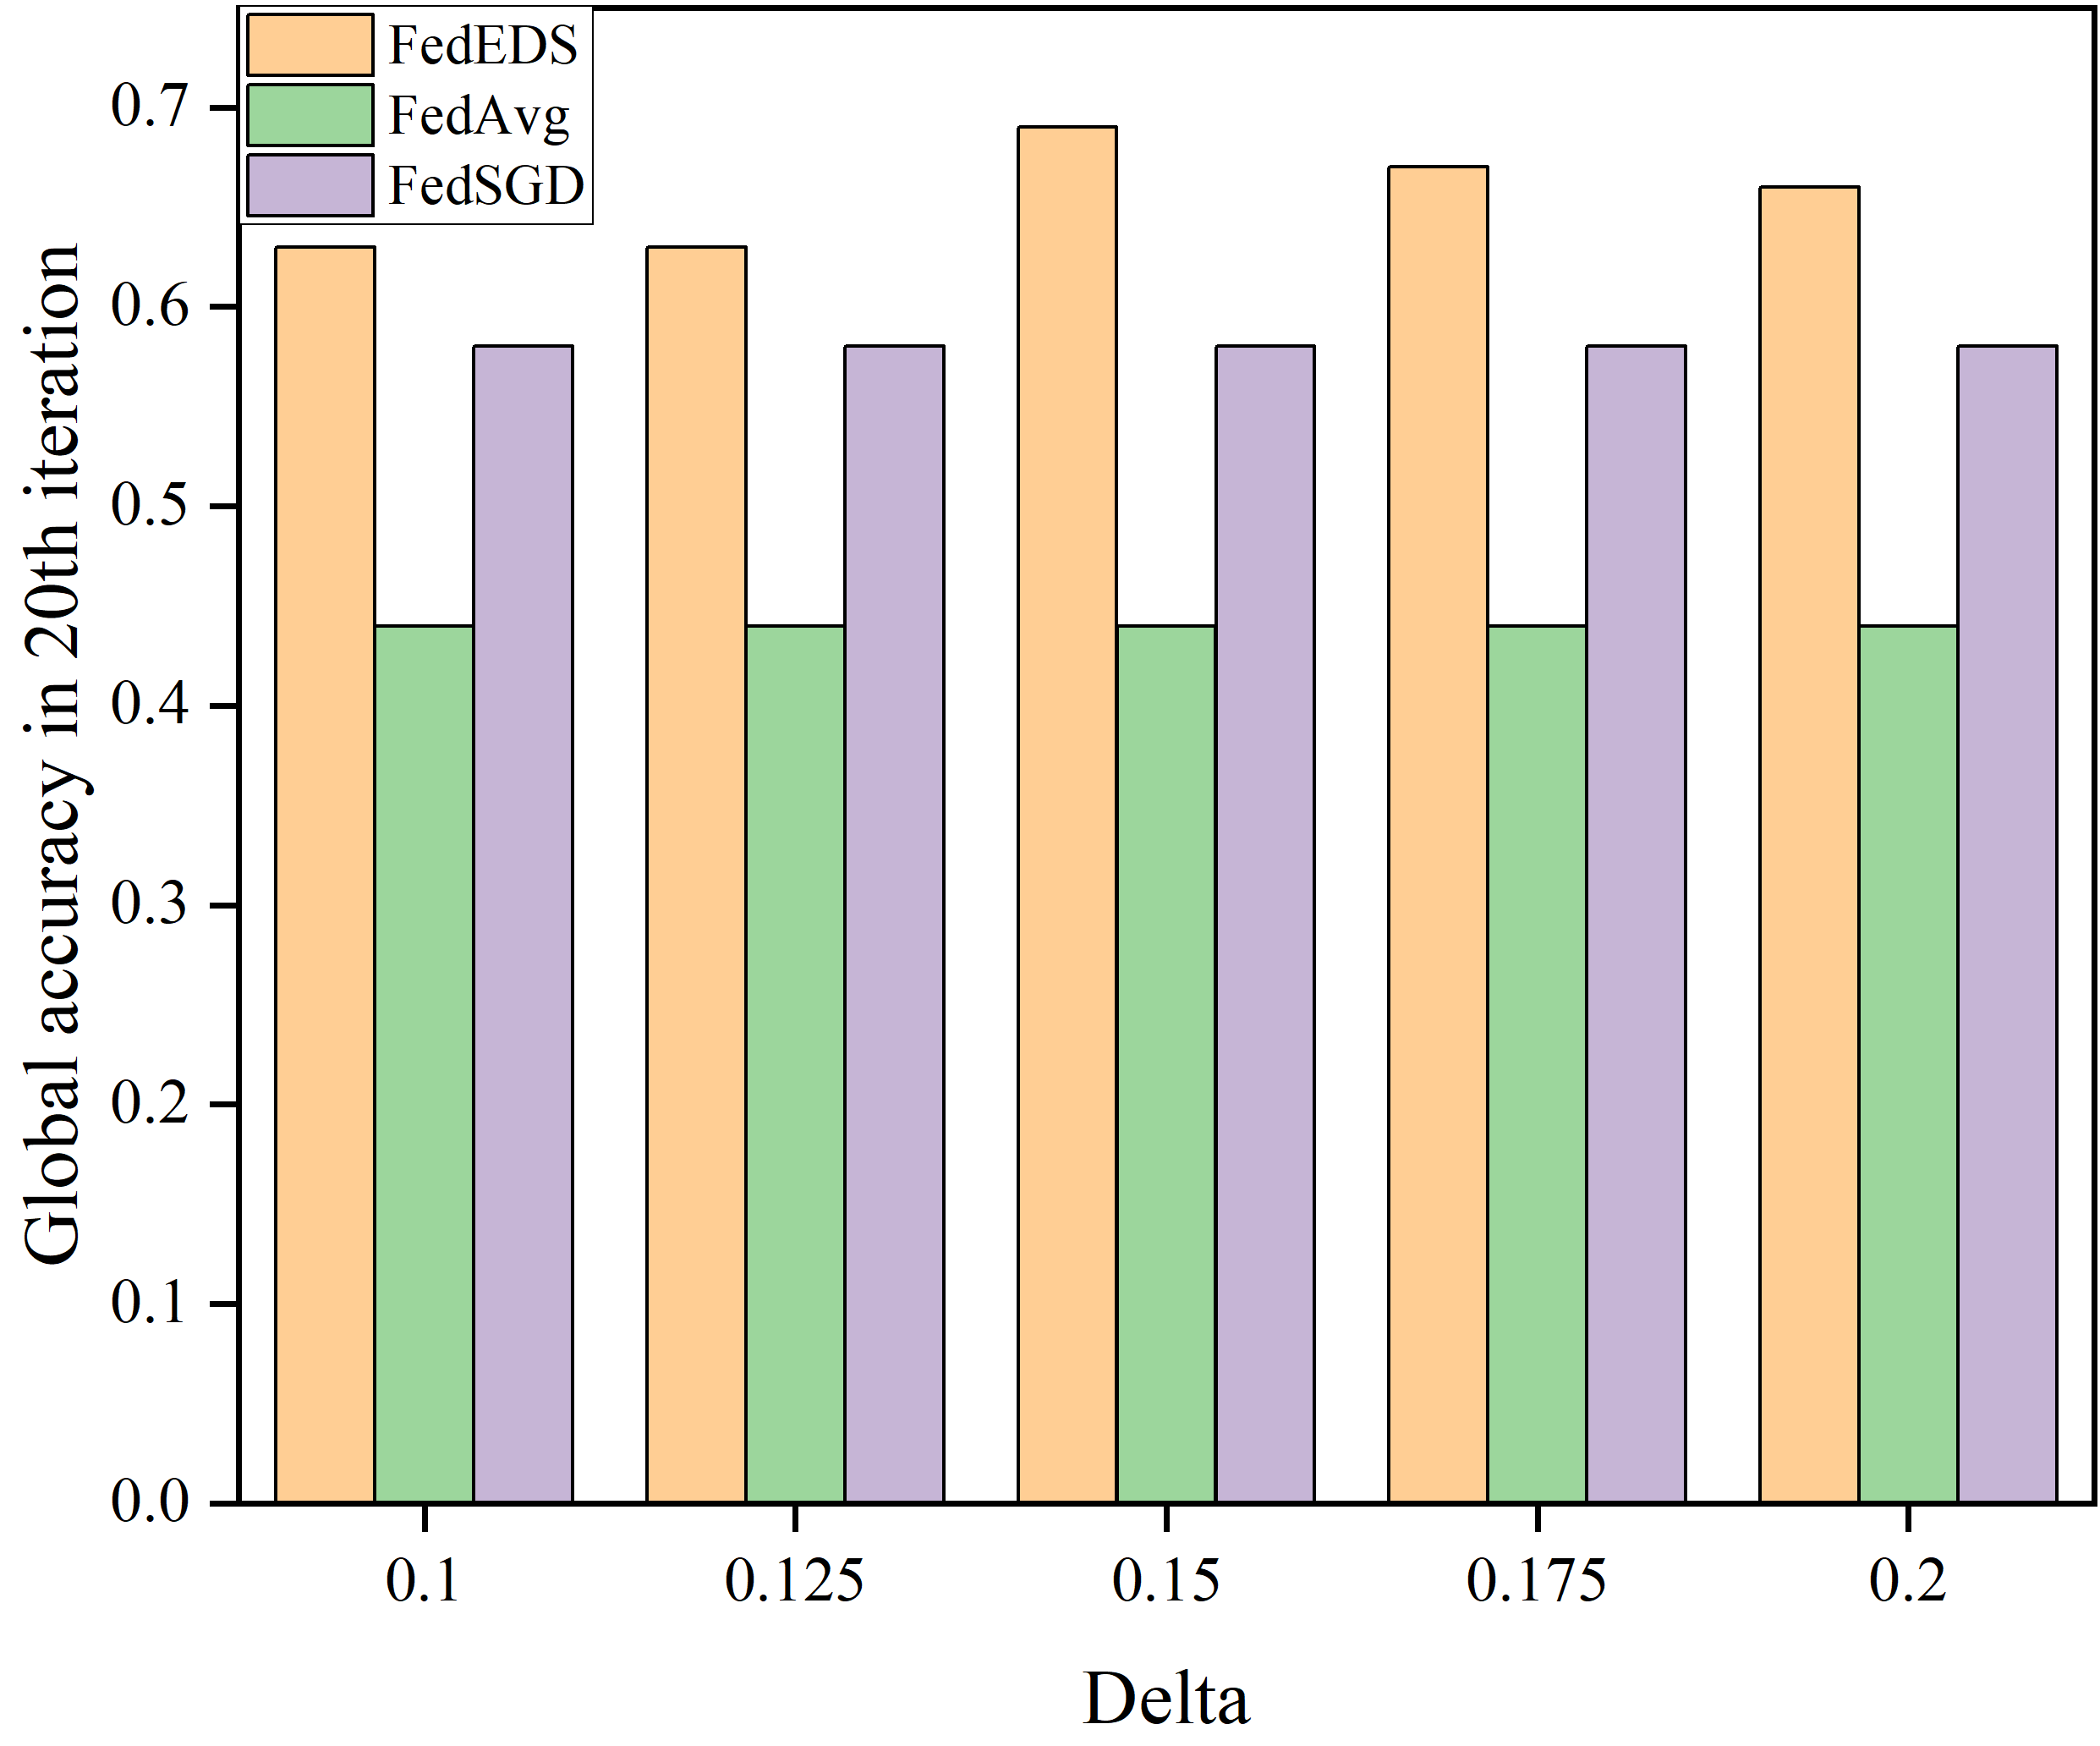
\includegraphics[height=3cm,width=4cm]{CIFAR_GROUP_AlexNet_PNG.png}
%     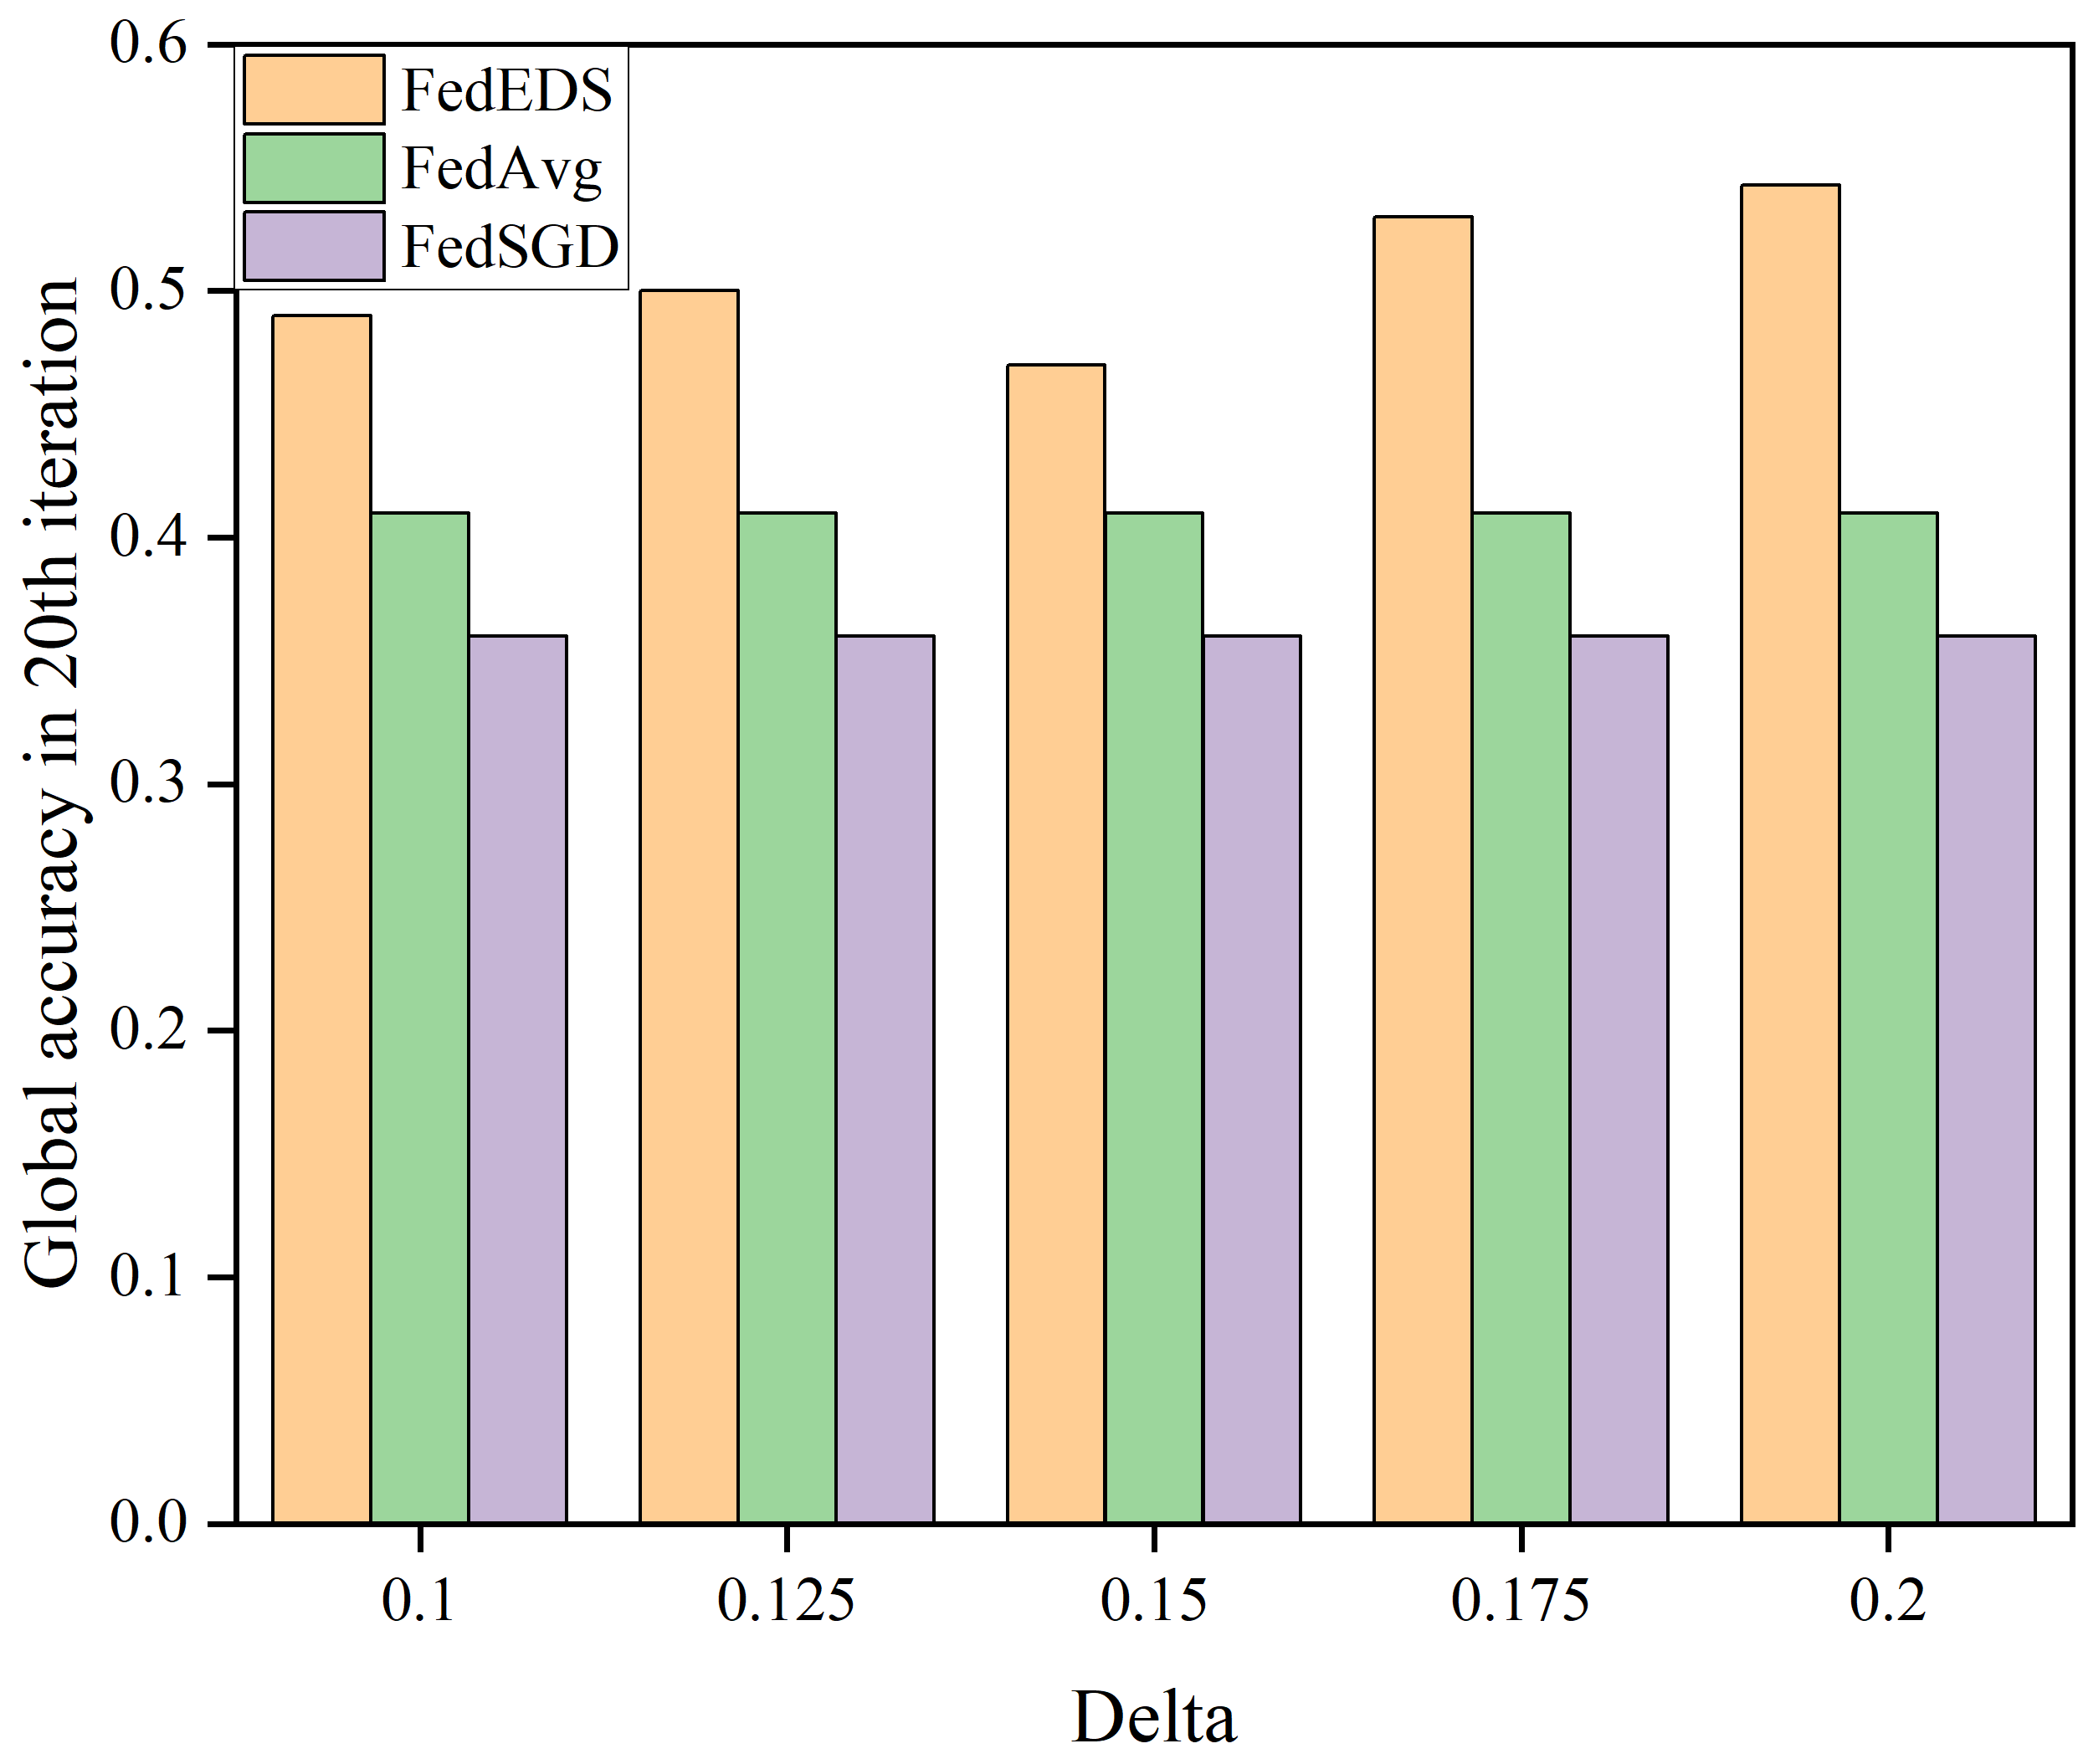
\includegraphics[height=3cm,width=4cm]{CIFAR_GROUP_LeNet_PNG.png}
%     \caption{Global Accuracy in Different $\delta_s$}
%     \label{MNINST}
% \end{figure}
\subsubsection{Environment Setting}
We utilize TensorFlow Federated (TTF) framework to simulate the server and client model.
Each client has similar level hardware: CPU-Intel Core 8700K, RAM-64GB, GPU-1080Ti 
(SLI, CUDA10.0), OS-Ubuntu20.04. TensorFlow-1.14.

Each client is allocated with an Intel CPU, which enables them to run the preset 
EM algorithm program in Enclave in parallel. Clients and server are deployed 
separately, they communicate through HTTP protocol. 
And the clients are distributed deployed, each client can only sense its own data.
In this paper we assume the total number of clients is 10, and we design different GMM on each client to 
stimulate the real-world distribution. Moreover, we set the local training iteration for different CNN and 
different data set. For CIFAR-10 with AlexNet and LeNet-5, we set the local iteration $l = 4$ and $l = 6$ respectively. 
And for MNIST with AlexNet and LeNet, we set $l = 2$ and $l=4$.
\subsection{Results on Practical  Non-IID data Setting}
\subsubsection{Estimation Results}
In this section, we bring out an experiment which aims to estimate parameters of 
a 3 branch GMM. We assume a 3-branch GMM follows probability function as follows
\begin{align}
  &p(x|\alpha,u,\sigma) = 0.572N(x|1.74,0.0865) \notag \\
  &+0.227N(x|1.63,0.062)+0.2N(x|2.1,0.001) \notag
\end{align}

We firstly generate a series of samples which follow the above function and denote
it as the observation data $x$. Then we execute the estimation algorithm for serval rounds. 
After the iterative calculation, we compare the results with the actual parameters. 
For a more intuitive view of the comparison results, we use 
$\frac{(\sum_{k}^{K}u_k – Ku_r)}{Ku_r}, k=\left\{1,2,\dots,K \right\}$ to calculate 
the average error ratio of the parameters and show the variation of the errors in each round. 

Obviously, through the algorithm, we get anideal result. Table 2 shows the 
estimation values in 400 rounds and figure 3 shows 
the difference between standard value and estimation value in 1000 rounds. 

The estimation algorithm runs on each independent device, while the apacity of calculation can be scarce,
the process reaches convergence in limited rounds and the convergence speed is also acceptable.

\subsubsection{Time Loss}
Since the estimation part is running in Intel SGX Enclave, we test the time consumption of 
executing algorithm under different data scales. We disabled automatic CPU frequency scaling,
Turbo Boost, and hyper-threading to avoid inconsistent performance behaviour.
We test the startup and shutdown overhead of Enclave in different buffer size, 
aiming to figure out the time loss of running program in SGX. We set the 
buffer size as 20kb, 10Mb, 40Mb and 160Mb, and record the consumed CPU cycles, table 2 shows the experiment result. 

While the upper limit of data size in each client is 600 (10\% of 6000),
which is far less than the 20kb, therefore, we can see that the time loss of Intel SGX is completely acceptable.

 
\subsubsection{Training Results}
We first test the global accuracy on 10 different clients, apparently, 
as shown in figure 4, FedDCS has higher global accuracy and faster convergence 
compared to FedAvg and FedSGD on both CIFAR-10 and MNIST datasets. 
Take CIFAR-10 with AlexNet for example, while the global accuracy of 
final convergence between FedSGD and FedDCS is very close, the FedDCS
 achieve a faster convergence. Then we test the accuracy of 
 FedDCS in different $\delta_s$ settings, and compare it with FedAvg 
 and FedSGD in the same rounds. Figure 5 shows the results, our method has better
  performance and the optimum threshold is 0.175.

\section{conclusion}
In this paper, we tackle the challenging problem of 
real-scene-based Non-IID data FL and develop 
FedDCS that introduces a parameter-estimation-based dynamic selection
mechanism to significantly facilitate the collaboration effectiveness
between clients without infringing their privacy. We analyze the 
distribution of real-world data and utilize GMM to build the Non-IID
data distribution model, which builds the foundation of the estimation
algorithm. Moreover, we introduce Intel SGX to keep data from privacy
leakage risk and conduct extensive experiments to prove the time loss is acceptable.

\newpage
\bibliographystyle{IEEEtran}
\bibliography{sample-base}
\end{document}
